\chapter{Spazi di Hilbert e teoria degli operatori}

Sia $\H$ uno spazio lineare su $\C$, cioè uno spazio nel quale sono definite la somma e il prodotto per uno scalare. Esso si dice \textbf{spazio pre-hilbertiano} se è definito  il \textbf{prodotto interno}, cioè un'operazione $\H \times \H \to \C$ : $(x|x) \geq 0$, e $(x|x) =0 \iff x=0$.\\Quando scambiamo due termini nel prodotto interno così definito, prendiamo il complesso coniugato del nuovo prodotto, cioè si ha che $(x|y)=\overline{(y|x)}$.
\\
Il prodotto interno così definito è lineare nel secondo membro e antilineare nel primo; infatti:

\begin{itemize}
\item $(x|\lambda y_1 + \mu y_2)=(x|\lambda y_1) + (x|\mu y_2) =\lambda (x|y_1) + \mu (x|y_2)$
\item $(\lambda x_1+\mu x_2|y)=\overline{(y|\lambda x_1 + \mu x_2)}=\overline{\lambda (y|x_1)+ \mu (y|x_2)} = \overline{\lambda} (x_1|y) + \overline{\mu} (x_2|y)$
\end{itemize} Vediamo ora le proprietà del prodotto scalare:

\begin{itemize}
\item $x$ è ortogonale a $y$ ($x \perp y$) se $(x|y)=0$
\item Introduciamo la quantità $\|x\|=\sqrt{(x|x)}$, che dimostreremo essere la norma; risultano ovvie alcune proprietà:
\begin{itemize}
\item $\|x\| \geq 0$
\item $\|x\| =0 \iff x=0$
\item $\| \lambda x\|=|\lambda| \|x\|$
\end{itemize}
\item Prendiamo $x,y$ tali che $x \perp y$; si ha che $\|x+y\|^2=\|x\|^2+\|y\|^2$. Infatti: 
$$\|x+y\|^2=(x+y|x+y)=(x|x)+(x|y)+(y|x)+(y|y)=\|x\|^2+\|y\|^2$$
Questa uguaglianza risulta quindi essere il \textbf{teorema di Pitagora}.
\item $u_k$, con $k=1,2, \dots ,N$ è un \textbf{sistema ortonormale} di vettori di $\H$ se $(u_k|u_j)=\delta_{kj}$
\item \textbf{Disuguaglianza di Bessel}: $\|x\|^2 \geq \sum_{k=1} ^N |(u_k|x)|^2$ \\
Dimostriamo questo fatto: chiamiamo $x'=\sum_{k=1} ^N (u_k|x)u_k$, e scriviamo $x$ come $(x-x')+x'$. Mostriamo che $(x-x'|x')=0$; una volta mostrato questo, si ha che: 
$$\|x\|^2 =\|x+x'\|^2 + \|x'\|^2 \geq \|x'\|^2 =(x'|x')= \sum_{k=1} ^N (u_k|x)(x'|u_k)=$$
$$=\sum_{k=1} ^N (u_k|x)(x|u_k)=\sum_{k=1} ^N |(u_k|x)|^2$$
Infatti si ha che 
$$(x'|u_k)=(\sum_{l=1} ^N (u_l|x) u_l|u_k)=\sum_{l=1} ^N \overline{(u_l|x)} (u_l|u_k)=\sum_{l=1} ^N (x|u_l) \delta_{lk}=(x|u_k)$$
Possiamo dimostrarlo anche partendo dalla condizione $(x-x'|x') =0$; infatti:
$$(x-x'|x')=(x|x')-(x'|x')=\sum_{k=1} ^N (u_k|x)(x|u_k)-\|x'\|^2=0$$
e da qui si ottiene la disuaglianza di Bessel.
\item \textbf{Disuguaglianza di Schwarz}: $|(x|y)|\leq \|x\| \|y\|$ \\Siano $x,y,\lambda$ dei numeri complessi; per ogni $\lambda$ si ha che: 
$$0 \leq \|x+\lambda y\|^2=(x+\lambda y|x+\lambda y)=\|x\|^2+|\lambda|^2 \|y\|^2 + \overline{\lambda}(y|x) + \lambda (x|y) \leq \footnote{Si usa la proprietà dei numeri complessi per la quale $\overline{x} + x =2  Re(x) \leq 2|x|$.}$$
$$\leq \|x\|^2 +|\lambda|^2 \|y\|^2 +2|\lambda||(x|y)|$$
Possiamo vedere tale risultato come un'equazione quadratica nella variabile $|\lambda|$; cerchiamo la condizione $\Delta \leq 0$:
$$|(x|y)|^2 - \|x\|^2 \|y\|^2 \leq 0 \implies |(x|y)|^2 \leq \|x\|^2 \|y\|^2$$
Utilizzando tale relazione per maggiorare il risultato precendente e ponendo $\lambda=1$ otteniamo che:
$$\|x+y\|^2 \leq  \|x\|^2 + \|y\|^2 +2|(x|y)|^2 \leq \|x\|^2 +\|y\|^2+2\|x\|^2 \|y\|^2=(\|x\| + \|y\|)^2$$
e quindi $\|x+y\| \leq \|x\|+\|y\|$, cioè la tesi.
\end{itemize} Quindi $\|x\|=\sqrt{(x|x)}$ è una \textbf{norma (hilbertiana)}, poichè valgono le seguenti proprietà:

\begin{itemize}
\item $\|x\| \geq 0$, e $\|x\|=0 \iff x=0$
\item$\| \lambda x\|=| \lambda| \|x\|$
\item Vale una disuguaglianza triangolare, cioè la disuguaglianza di Schwarz
\end{itemize} Le proprietà della norma hibertiana sono:

\begin{itemize}
\item $\|x \pm y\|^2= \|x\|^2 +\|y\|^2 \pm Re((x|y))$
\item Vale la \textbf{proprietà del parallelogrammo}, cioè si ha che $\|x+y\|^2+\|x-y\|^2=2\|x\|^2 + 2 \|y\|^2$
\end{itemize}

\begin{teorema}

Condizione necessaria e sufficiente affinchè una norma sia  hilbertiana (cioè che discenda da un prodotto interno) è che valga la proprietà  del parallelogrammo.
\end{teorema}

\begin{proof} Se la norma è hilbertiana, la dimostrazione è ovvia.

Se vale la proprietà del parallelogrammo, si dimostra che $\frac{1}{4} (\|x+y\|^2-\|x-y\|^2)$ e  $\frac{1}{4} (\|x-iy\|^2-\|x+iy\|^2)$ sono rispettivamente la parte reale e la parte immaginaria in un prodotto interno $(x|y)$; a questo punto, verificando le proprietà del prodotto interno, si ricava che quello appena definito è un prodotto interno solo se vale la proprietà del parallelogrammo.

\end{proof}

La formula del prodotto interno definita nella dimostrazione è detta \textbf{formula di polarizzazione} ed è qui riportata integralmente:
$$(x|y)= \frac{1}{4} (\|x+y\|^2-\|x-y\|^2)+ \frac{i}{4} (\|x-iy\|^2+\|x+iy\|^2)$$
Uno spazio con prodotto interno è detto \textbf{spazio normato}; se è completo (cioè se tutte le successioni di Cauchy sono convergenti), lo spazio è detto \textbf{spazio di Hilbert}\footnote{La sistematizzazione degli spazi di Hilbert è dovuta a Von Neumann.}.
\\
\\
L'operazione prodotto interno $(x|\, \cdot):\H \to \C$ è un'applicazione lineare ed è continua; se una successione $y_n$ converge a $y$ in $\H$, allora il prodotto interno $(x|y_n)_{\C}$ converge a $(x|y)$. Cosa vuol dire che la successione converge? Vuol dire che la quantità $|(x|y_n)-(x|y)|$ tende a $0$; infatti possiamo scrivere che $|(x|y_n)-(x|y)|=|(x|y_n-y)|$ e, per la disuguaglianza di Schwarz, si ha che $|(x|y_n-y)| \leq \|x\| \|y_n-y\|$ e, dato che $y_n \to y$, si ha che il tutto tende a $0$. \\Quello che abbiamo appena analizzato è un esempio di \textbf{funzionale lineare continuo}, cioè un'applicazione lineare a valori in $\C$ e continua. \\Quindi il prodotto interno $(x|\, \cdot) \in \H^*$, cioè appartiene all'insieme dei funzionali lineari continui di $\H$ (detto \textbf{duale di $\H$}).

Tutti gli elementi di $\H^*$ sono della forma $(x|\, \cdot)$, cioè gli elementi del duale di $\H$ sono in corrispondenza biunivoca con gli elementi di $\H$.
\\
Due spazi di Hilbert $\H_1$ e $\H_2$ si dicono \textbf{isomorfi} se esiste una mappa $\hat{U}:\H_1 \to \H_2$ lineare invertibile; inoltre, tale $\hat{U}$ conserva la norma, cioè $\|\hat{U} x \|_2=\|x\|_1$ $\forall x \in \H_1$. \\Per effetto della formula di polarizzazione, si ha che siffatta mappa conserva il prodotto interno, cioè $(\hat{U} x|\hat{U}y)_2=(x|y)_1$ $\forall x,y$; tale proprietà è detta \textbf{isomorfismo hilbertiano}.

L'operatore $\hat{U}$ è un \textbf{operatore lineare unitario}. Tutte le simmetrie continue sono rappresentate da operatori unitari.
\\
\\
Esempi:
\begin{itemize}
\item Gli insiemi $\R^n$ e $\C^n$ in cui il prodotto interno è definito come il prodotto scalare, cioè in cui $(u|v)=\sum_k u_k v_k$
\item L'insieme $\C^{n \times n}$, cioè l'insieme delle matrici $n \times n$ a coefficienti complessi, in cui il prodotto interno è definito come $(A|B)=Tr(A^+ B)$; l'operatore ''$^+$'' indica che viene presa la matrice trasposta coniugata, cioè si ha che $(A^+)_{ij}=\overline{A}_{ji}$.
\end{itemize}

Introduciamo ora lo spazio $l^2(\C)$, cioè lo spazio delle successioni numeriche in $\C$ tali che la serie dei quadrati converga; quindi un elemento  $a \in l^2(\C)$ e una successione $\{ a_n\}_{n=0} ^{\infty}$ tale che ogni $a_n \in \C$ e $\sum_k |a_n|^2 < \infty$. Lo spazio $l^2(\C)$ è uno spazio lineare, poichè valgono: 
\begin{itemize}
\item $a,b \in l^2(\C) \implies a+b=\{a_n + b_n\} \in l^2(\C)$
\item $a \in l^2(\C) \implies \lambda a=\{ \lambda a_n\} \in l^2(\C)$
\end{itemize}
Il prodotto interno per lo spazio $l^2(\C)$ è definito come:
$$(a|b) = \sum_{n=0} ^{\infty} \overline{a_n} b_n$$
e quindi la norma quadra di un elemento $a \in l^2(\C)$ è definita come:
$$\sum_{n=0} ^{\infty} |a_n|^2 < \infty$$
Per verificare che quello definito sopra sia un prodotto interno, bisogna verificare che la serie converge $\forall a,b \in l^2(\C)$.
\\
\\
\\
Dimostriamo ora il seguente teorema:
\begin{teorema}
Lo spazio $l^2(\C)$ è completo, cioè ogni successione di Cauchy converge.
\end{teorema}
\begin{proof}
Sia $a_n$ una successione di Cauchy; vale allora che
$$\forall \epsilon >0 \text{ } \exists N_{\epsilon} \text{ : } \|a_n-a_m\|_2 <\epsilon \text{ } \forall n,m>N_{\epsilon}$$
Quindi possiamo scrivere:
$$\|a_n-a_m\|^2= \sum_{k=0} ^{\infty} |a_n ^{(k)} - a_m ^{(k)}|^2 < \epsilon ^2 \implies \forall |a_n ^{(k)} - a_m ^{(k)}|^2 < \epsilon ^2 \text{ } \forall n,m>N_{\epsilon}, \forall k=0,1,2,\dots$$
Allora abbiamo costruito una successione\footnote{La successione è di indice n; l'indice k ci serve per definire la successione dei limiti.} $a_n ^{(k)}$ che è di Cauchy e converge ad un certo $a^{(k)}$ $\forall k$\footnote{Si ha cioè che $a_n ^{(1)} \to a^{(1)}, a_n ^{(2)} \to a^{(2)} \dots$}. Presa la successione di tali limiti, cioè $\{a^{(k)}\}$, sia $a$ il limite di tale successione. Per $m \to \infty$, si ha che:
$$\sum_{k=0} ^{\infty} |a_n ^{(k)} - a_m ^{(k)}|^2= \sum_{k=0} ^{\infty} |a_n ^{(k)} - a^{(k)}|^2 < \epsilon ^2$$
Dato che $a_n \in l^2(\C)$ e dato che l'elemento $|a_n -a|$ appartiene a $l^2(\C)$, per linearità si ha che  anche $a \in l^2(\C)$. Poichè $a_n \to a$, si ha la tesi.

\end{proof}

\section{Lo spazio $\L^p (\Omega)$}

Lo spazio  $\L^p (\Omega)$, dove $\Omega$ è un'insieme misurabile, è uno spazio di funzioni per le quali vale che
$$\int dx |f|^p < \infty$$
La norma in tale spazio vale:
$$\|f\| _p=\sqrt[p]{\int dx |f|^p}$$
Introduciamo ora due importanti risultati:
\begin{itemize}
\item \textbf{Disuguaglianza di H\"{o}lder} \\Siano $f \in \L^p (\Omega)$ e $g \in \L^q (\Omega)$, con $\frac{1}{p} + \frac{1}{q} =1$; allora si ha che \\$$\int_{\Omega} |fg|dx \leq \|f\|_p \|g\|_q$$
\item \textbf{Disuguaglianza di Minkowski} \\Siano $f, g \in  \L^p (\Omega)$. Allora si ha che \\$$\|f+g\|_p \leq \|f\|_p + \|g\|_p$$
\end{itemize}
Non dimostreremo queste due disuguaglianze, ma le citiamo perchè da esse possiamo ricavare delle importanti proprietà; infatti, dalla disuguaglianza di Minkowski ricaviamo che:
\begin{itemize}
\item Siano $f,g \in \L^p (\Omega)$; allora si ha che anche $f+g \in \L^p (\Omega)$
\item Sia $f \in \L^p (\Omega)$ e sia $\lambda \in \C$; allora si ha che $\lambda f \in \L^p (\Omega)$
\end{itemize}
Cioè otteniamo che lo spazio $\L^p (\Omega)$ è lineare.
Dovremmo quindi dimostrare le tre proprietà degli spazi lineari:
\begin{itemize}
\item $\| \lambda f\|_p=|\lambda| \|f\|_p$
\item $\|f+g\|_p \leq \|f\|_p + \|g\|_p$
\item $\|f\|_p \geq 0$
\end{itemize}
Prima di tutto però ci chiediamo: vale che $\int dx |f|^p =0 \iff f=0$? Non vale, altrimenti si avrebbe che $f=0$ q.o.\footnote{q.o. è l'abbreviazione di ``quasi ovunque'', che significa che la proprietà citata vale sempre tranne che in insiemi di misura nulla.} (e per gli integrali gli insiemi di misura nulla non contano, cioè il contributo di un insieme di misura nulla ad un integrale è zero). \\Come risolviamo questo problema? Introduciamo una relazione di equivalenza $f \sim g$ che mette in relazione le funzioni $f$ e $g$ se si ha che $f=g$ q.o.; possiamo quindi dividere le funzioni per classi di equivalenza $[f]$. \\Prese due classi di equivalenza $[f]$ e $[g]$, ognuna di esse avrà un rappresentante (che indicheremo rispettivamente con $f$ e $g$); abbiamo che valgono le proprietà di linearità, cioè si ha che $[f]+[g]=[f+g]$ e $\lambda [f]=[\lambda f ]$.

Tutti gli elementi di una stessa classi di equivalenza hanno la stessa norma a p ($\|$ $\|_p$); oltretutto, quando si ha che $\|f\|_p=0$, allora l'intera classe di equivalenza $[f]$ è l'elemento nullo.

Quindi l'insieme $\L^p (\Omega)$ contiene classi di equivalenza di funzioni misurabili, con $\int_{\Omega} dx |f|^p < \infty$. Esso è uno spazio lineare (per quanto visto prima), ed è anche normato con $\|f\|_p=\sqrt[p]{\int_{\Omega} dx |f|^p}$. Inoltre uno spazio di questo tipo (con $p \geq 1$) è uno spazio completo, cioè $f_n \to f$ in $\L^p (\Omega)$ se $\|f_n-f\|_p \to 0$.
\begin{teorema} (di Fisher-Riegz)\\
$\L^p (\Omega)$ è uno spazio completo (\textbf{spazio di Banach}) se $p \geq 1$.
\end{teorema}
Noi useremo principalmente due di questi spazi: lo spazio $\L^1 (\Omega)$, cioè lo spazio delle funzioni integrabili (infatti si ha che la condizione sulla norma rappresenta la condizione di integrabilità, $\|f\|_1 =\int_{\Omega} dx |f| < \infty$), e lo spazio $\L^2 (\Omega)$; per quest'ultimo, abbiamo la particolarità del fatto che la norma che abbiamo definito è una norma hilbertiana, perchè si ha $\|f\|_2=\sqrt{\int_{\Omega} dx |f|^2} < \infty$. Quindi lo spazio $\L^2 (\Omega)$ è uno spazio di hilbert, con prodotto interno definito come:
$$(f|g)=\int_{\Omega} \overline{f} g dx$$
dove abbiamo preso i rappresentanti delle due classi di equivalenza $[f]$ e $[g]$.

\begin{osservazione} Se la misura dell'insieme $\Omega$ è finita, cioè se si ha che $\mu (\Omega) < \infty$, allora la funzione $f=cost$ $\in \L^p (\Omega)$. Sia infatti $\int_{\Omega} 1 |f| dx$, con $\mu(\Omega) < \infty$, e supponiamo che $f \in \L^2 (\Omega)$; allora si ha che:
$$\|f\|_1=\int_{\Omega} 1 |f| dx=(1|f)_2 \leq \footnote{Per la disuguaglianza di Schwarz} \|1\|_2 \|f\|_2$$
dove $\|1\|_2$ è proprio la misura $\mu(\Omega)$ che è finita; quindi se $f \in \L^2 (\Omega)$ ai ha anche che $f \in \L^1 (\Omega)$.
\end{osservazione}

\section{Sistemi ortogonali}

Sia $\H$ uno spazio di Hilbert qualunque, e sia $\mathcal{M}$ un suo sottoinsieme. Esso è un sottospazio se è chiuso per addizione e moltiplicazione per uno scalare in $\C$. In più, $\mathcal{M}$ è un sottospazio chiuso se, qualora si abbia che $x_n \to x$ con $x_n \in \mathcal{M}$, allora $x \in \mathcal{M}$.\\
Inoltre, possiamo definire il complemento ortogonale del sottospazio $\mathcal{M}$:
$$\mathcal{M}^{\perp}=\left\{x \in \H \, : \, (x|y)=0 \, \, \forall y \in \mathcal{M} \right\}$$
Risulta abbastanza semplice verificare che $\mathcal{M}^{\perp}$ è un sottospazio lineare; infatti:
\begin{itemize}
\item $x, x' \in \mathcal{M}^{\perp} \implies x+x' \in \mathcal{M}^{\perp}$
\item $x \in \mathcal{M}^{\perp} \implies \lambda x \in \mathcal{M}^{\perp}$
\end{itemize}
Oltretutto, abbiamo che $\mathcal{M}^{\perp}$ è chiuso:
\begin{teorema}
Sia $x_n$ una successione in $\mathcal{M}^{\perp}$, con $x_n \to x$; allora $x \in \mathcal{M}^{\perp}$.
\end{teorema}
\begin{proof}
La dimostrazione è immediata; infatti per definizione di complemento ortogonale, abbiamo:
$$(x_n|y)=0 \, \, \forall y \in \mathcal{M}, \, \forall n$$
Poichè la norma $( \cdot |y)$ è un operatore continuo, deve essere che $(x|y)=0$; ma allora $x \in  \mathcal{M}^{\perp}$, cioè $\mathcal{M}^{\perp}$ è chiuso.
\end{proof}
Possiamo dimostrare questo fatto anche partendo dalla proprietà per cui, dato un insieme $\mathcal{M}$, si ha che il complemento ortogonale del complemento ortogonale è $(\mathcal{M}^{\perp})^{\perp}=\overline{\mathcal{M}}$; però esso deve anche coincidere con l'insieme $\mathcal{M}$ e, dato che la proprietà vale per ogni $\mathcal{M}$, otteniamo che il complemento ortogonale è per forza chiuso.
\begin{definizione}
Si definisce la distanza di un elemento $x$ dall'insieme $\mathcal{M}$ la quantità
$$d(x,\mathcal{M})= \inf_{y \in \mathcal{M}} \|x-y\|$$
\end{definizione}
\begin{teorema}
Sia $\mathcal{M}$ un sottospazio chiuso e sia $x$ un elemento qualunque di $\H$. Allora esiste unico $p \in \mathcal{M}$ tale che $d(x,\mathcal{M}) = \|x-p\|$
\end{teorema}
\begin{teorema}
Sia $\mathcal{M}$ un sottospazio chiuso di $\H$ e sia $x \in \H$. $x$ si può scrivere in maniera unica come $x=x_1 + x_2$, con $x_1 \in \mathcal{M}$ e $x_2 \in \mathcal{M}^{\perp}$.
\end{teorema}
\begin{proof}
Sia $x_1=p \in \mathcal{M}$; per il teorema precendente, vale che  $d(x,\mathcal{M})=\|x-p\|$; dobbiamo dimostrare che $x-p \in \mathcal{M}^{\perp}$.\\
Consideriamo la norma $\|x-p-\lambda y\|^2$, dove $y \in \mathcal{M}$ e $\lambda \in \C$. Possiamo scrivere:
$$\|x-p\|^2 \leq \|x-p-\lambda y\|^2 = (x-p- \lambda y|x-p-\lambda y)=\|x-p\|^2 + |\lambda |^2 \|y\|^2 -2Re[\lambda (x-p|y)]$$
Quindi confrontanto il primo e l'ultimo membro, otteniamo:
$$0 \leq  |\lambda |^2 \|y\|^2 -2Re[\lambda (x-p|y)] \text{ } \forall \lambda , \, \forall y \in \mathcal{M}$$
Richiedere che la disequazione valga $\forall \lambda$ ci permette di scrivere che allora $(x-p|y)=0$, cioè $x-p \in \mathcal{M}^{\perp}$ (perchè abbiamo supposto $y \in \mathcal{M}$).\\
\\
Per dimostrarne l'unicità, procediamo per assurdo; ipotizziamo che l'elemento $x$ possa essere scritto simultaneamente come $x_1-x_2$ e $\tilde{x}_1 - \tilde{x}_2$, con i primi elementi appartenenti a $\mathcal{M}$ e i secondi appartenenti a $\mathcal{M}^{\perp}$; valutiamo la differenza fra le due scritture:
$$0=(x_1- \tilde{x}_1)+(x_2-\tilde{x}_2)$$
Per la struttura di $\mathcal{M}$, abbiamo che la prima parentesi è ancora un elemento di $\mathcal{M}$ e similmente la seconda è un elemento di $\mathcal{M}^{\perp}$; valutando la norma:
$$0=\|(x_1- \tilde{x}_1)+(x_2-\tilde{x}_2)\|^2=\|x_1- \tilde{x}_1\|^2+\|x_2-\tilde{x}_2\|^2$$
e quindi, si deve avere che $x_1= \tilde{x}_1$ e $x_2=\tilde{x}_2$.
\end{proof}
\begin{definizione}
Siano $\mathcal{M}_1, \mathcal{M}_2$ due sottospazi lineari chiusi di $\mathcal{M}$ ortogonali fra di loro. La somma ortogonale dei due sottospazi, definita come:
$$\mathcal{M}_1 \oplus \mathcal{M}_2=\left\{x \text{ : } x=x_1+x_2\text{, con } x_1 \in \mathcal{M}_1 \text{ e } x_2 \in \mathcal{M}_2 \right\}$$
è un sottospazio chiuso.
\end{definizione}
Grazie a questa definizione, possimamo ridimostrare il teorema precedente; infatti, abbiamo che un qualsiasi spazio di Hilbert può essere decomposto nella somma (ortogonale) di tanti sottospazi ortogonali, cioè possiamo sempre scrivere $\H=\mathcal{M} \oplus \mathcal{M}^{\perp}$.
\\
\\
Sia $\mathcal{M}$ sottospazio chiuso e sia $x$ associato a $p \in \mathcal{M}$. Definiamo l'operatore di proiezione $\hat{P}: \H \to \H$ come l'operatore la cui azione su $x$ è $\hat{P} x=p$ cioè l'operatore che porta $x \mapsto p$. L'operatore $\hat{P}$ è detto \textbf{proiettore ortogonale di $\mathcal{M}$}.\\
Vediamo alcune proprietà di $\hat{P}$:
\begin{itemize}
\item $\hat{P}$ è lineare, cioè vale che $\hat{P}(\lambda x + \tilde{x})=\lambda \hat{P}x+\hat{P} \tilde{x}$
\item $\hat{P}^2=\hat{P}$; questa è detta \textbf{proprietà di idempotenza}
\item il dominio di $\hat{P}$ è tutto $\H$; l'immagine di $\hat{P}$ è il sottospazio $\mathcal{M}$ mentre il kernel è l'insieme $\\ker \hat{P} = \left\{ x \text{ : } \hat{P}x=0 \right\}$, cioè l'insieme $\mathcal{M}^{\perp}$
\item Il proiettore contrae o lascia invariata la norma di un vettore; infatti, scomponendo il generico elemento $x$ come visto in precedenza, abbiamo che:
$$\|x\|^2=\|p\|^2+\|y\|^2 \geq \|p\|^2 = \| \hat{P}x \|^2 \implies \| \hat{P}x \| \leq \|x\|$$
\item $\hat{P}$ è un operatore \textbf{autoaggiunto}; infatti, $\forall x, y \in \H$ abbiamo che:
$$(x- \hat{P}x|y- \hat{P}y)=(x-\hat{P}x|y) \text{ e allo stesso modo } (x- \hat{P}x|y- \hat{P}y)=(x|y-\hat{P}y)$$
quindi dalle precedenti uguaglianze otteniamo che:
$$(\hat{P}x|y)=(x|\hat{P}y)$$
\end{itemize}
Altri esempi di operatori sono:
\begin{itemize}
\item Nello spazio $\L^2(\R)$, cioè nello spazio delle funzioni a quadrato sommabile, possiamo scrivere una qualsiasi funzione $f: \R \to \R$ come somma della sua parte pari e della sua parte dispari, cioè $f=f_P + f_D$, dove $f_P =\frac{f(x)+f(-x)}{2}$ e $f_D =\frac{f(x)-f(-x)}{2}$; è facile verificare che $(f_P|f_D)=0$, cioè che possiamo scrivere il corrispettivo spazio di Hilbert come somma ortogonale di due sottospazi: $\H=\H_P \oplus \H_D$.\\Definiamo allora l'\textbf{operatore di parità $\hat{\pi}$}, la cui azione su una funzione $f$ è:
$$(\hat{\pi}f)(x)=f(-x)$$
Tale operatore ha autovalore $1$ se $f$ è pari, mentre ha autovalore $-1$ se $f$ è dispari; è facile verificare che il quadrato dell'operatore parità è l'identità. Possiamo inoltre definire un'operatore che restituisca la parte pari della funzione $f$ utilizzando l'operatore parità e l'identità; tale operatore è scritto come $\frac{\mathbb{I} + \hat{\pi}}{2}$. 
\item Sempre nello spazio $\L^2(\R)$, definiamo gli \textbf{operatori di moltiplicazione} che hanno azione sulla generica funzione $f \mapsto \phi f$, dove $\phi \in \L^2(\R)$. Nel momento in cui $\phi = \chi _{[a,b]}$, l'operatore ad essa associato è lineare, rispetta la proprietà di idempotenza ed è autoaggiunto; quest'ultima proèprietà si dimostra applicando la definizione di prodotto interno nello spazio $\L^2(\R)$.
\end{itemize}
%%%manca una parte (fine del foglio 39, retro)%%%
Sia dato l'operatore $\hat{A}:X \to Y$, con $X, Y$ spazi normati. Tale operatore si dice \textbf{lineare} se $\hat{A}(x_1 + \lambda x_2)=\hat{A}x_1 + \lambda \hat{A}x_2$. Introduciamo ora la nozione di limitatezza dell'operatore:
\begin{definizione}
$\hat{A}$ si dice  \textbf{limitato} se esiste $C_A >0$ tale che $\| \hat{A}x \|_{Y} \leq C_A \| x \|_{X} \, \, \forall x \in X$, cioè se si verifica che:
$$\frac{\| \hat{A}x \|_{Y}}{ \| x \|_{X}}\leq C_A$$
\end{definizione}
Cerchiamo tale costante:
$$\sup_{x \in X, x \neq 0} \frac{\| \hat{A}x \|_{Y}}{ \| x \|_{X}} = \| \hat{A} \|$$
quindi, grazie a questa definizione, possiamo sempre scrivere che $\| \hat{A}x \|_{Y} \leq \| \hat{A} \| \, \| x \|_{X}$.
Dati i due spazi normati $X, Y$, possiamo definire lo spazio $\mathcal{B}(X,Y)$, cioè l'insieme degli operatori limitati con dominio $X$ e codominio $Y$; in questo spazio, definiamo la somma di due operatori e il prodotto per uno scalare come:
$$(\hat{A} + \hat{B})x=\hat{A}x + \hat{B}x \text{ e } (\lambda \hat{A})x = \lambda (\hat{A}x)$$
Perchè $\mathcal{B}$ sia uno spazio, dobbiamo verificare che gli operatori qui sopra definiti sono anch'essi limitati; mostriamolo per la somma e per il prodotto per uno scalare il ragionamento è simile:
$$\| (\hat{A} + \hat{B})x \|_Y \leq  (\| \hat{A} \| + \| \hat{B}\| ) \|x\|_X \, \, \, \forall x$$
Dimostriamo ora che $\| \hat {A} \|$ è effettivamente una norma:
\begin{itemize}
\item $ \| \hat{A} \| = \sup_{x \in X, x \neq 0} \frac{\| \hat{A}x \|_{Y}}{ \| x \|_{X}}$
\item Possiamo ricavare uan disuguaglianza triangolare dalla dimostrazione della limitatezza della somma di due operatori
\item Una successione di operatori $\hat{A}_n$ converge all'operatore $\hat{A}$ in $\mathcal{B}$ se $\|\hat{A}_n - \hat{A} \| \to 0$ per $n \to \infty$; quindi lo spazio $\mathcal{B}$ non solo è uno spazio normato, ma è anche uno spazio di Banach.
\end{itemize}
\begin{teorema}
Se $Y$ è completo, allora $\mathcal{B}(X,Y)$ è completo.\\Se $\hat{A}$ è limitato, allora $\hat{A}$ è continuo.
\end{teorema}
Dobbiamo mostrare che se $x_n \to x$ in $X$, allora $\hat{A}x_n \to \hat{A}x$ in $Y$; similmente, ma utilizzando le norme, dobbiamo mostrare che $\|x_n - x \|_X \to 0 \implies \|\hat{A}(x_n-x)\|_Y \to 0$.
Per un operatore lineare la continuità per $x_n \to x$ è equivalente alla continuità per $x_n \to 0$; infatti, abbiamo che:
$$\|\hat{A}(x_n-x)\| \leq \|\hat{A}\| \, \|x_n-x\| \o 0$$
\begin{teorema}
L'operatore lineare $\hat{A}$ è continuo $\iff$ $\hat{A}$ è continuo in $x=0$.
\end{teorema}
Nel caso in cui gli insiemi $X$ e $Y$ siano lo stesso insieme, cioè nel caso in cui ci troviamo nello spazio $\mathcal{B}(X,X)$, possiamo definire il prodotto fra due operatori come:
$$(\hat{A} \hat{B})x=\hat{A}(\hat{B}x)$$
Passando alla norma, abbiamo la seguente disuguaglianza:
$$\| \hat{A} \hat{B} \| \leq \| \hat{A} \| \, \| \hat{B} \|$$
Ricaviamo tale disuguaglianza; per le proprietà della norma, vale che:
$$\| (\hat{A} \hat{B})x \|_X=\| \hat{A}(\hat{B}x)\|_X \leq \| \hat{A}\| \, \|\hat{B}x\|_X \leq \| \hat{A}\| \, \|\hat{B}\| \, \|x\|_X \, \, \forall x \implies \frac{\| (\hat{A} \hat{B})x \|_X}{\|x\|_X } \leq \| \hat{A}\| \, \|\hat{B}\| \, \, \forall x$$
Facendo il $\sup$, otteniamo il risultato scritto sopra.
\clearpage
Trattiamo ora lo spazio $\mathcal{B}(\H, \H)=\mathcal{B}(\H)$; possiamo definirne il duale $\H^*=\mathcal{B}(\H, \C)$, cioè lo spazio dei funzionali lineari continui su $\H$. Alcuni elementi di $\mathcal{B}(\H)$ sono:
\begin{itemize}
\item Gli operatori $\hat{P}$ tali che $\| \hat{P}x \| \leq \|x\|$, cioè tali per cui
$$\| \hat{P} \|= \sup_{x \neq 0} \frac{\| \hat{P}x \|}{\|x\|}=1$$
\item Gli operatori unitari $\hat{U}$, cioè quegli operatori tali che  $\| \hat{U}x \| = \|x\|$ $\forall x$; questa proprietà implica che anch'essi hanno norma unitaria.
\end{itemize}

\subsection{Esponenziale di un operatore}
\dots \dots \dots

\section{Basi ortonormali}
Un sistema ortonormale di vettori $\{u_a\}_{a \in A}$ (dove gli $u_a$ sono vettori dello spazio di Hilbert) è un sistema ortonormale completo (sonc) se:
$$(u_a|x)=0 \, \, \forall a \in A \implies x=0$$
Tale definizione ci permette di ottenere i seguenti risultati:
\begin{itemize}
\item Il sonc non è sottoinsieme  di un insieme ortonormale, cioè non possiamo aggiungere un vettore ortogonale a quelli già esistenti, poichè altrimenti avremmo per tale vettore (non nullo) che il prodotto interno con gli $u_a$ è nullo, contro le ipotesi.
\item La varientà lineare\footnote{La varientà lineare è l'insieme delle combinazioni lineare degli elementi di un insieme.} del sonc è lo spazio di Hilbert; in formule, $Var\{u_a\}_{a \in A}=\H$.
\end{itemize}
\begin{teorema}
Ogni spazio di Hilbert ammette un sonc $\{u_a\}_{a \in A}$.
\end{teorema}
Ogni elemento dello spazio di Hilbert può essere scritto come combinazione lineare degli elementi del sonc, secondo la formula:
$$x=\sum_{a \in A} (u_a|x)u_a$$
Oltretutto, vale l'\textbf{identità di Parseval}, che ridefinisce la norma di un elemento:
$$\|x\|^2 = \sum_{a \in A} |(u_a|x)|^2$$
Se lo spazio di Hilbert ammette un sonc numerabile, allora lo spazio è separabile\footnote{Uno spazio si dice separabile quando ammette un sottoinsieme numerabile denso, cioè la cui chiusura mi dia lo spazio di partenza.} ed è isomorfo a $\L^2(\C)$.\\
Prendiamo lo spazio $\L^2([a;b])$, con $b>a$; esso è lo spazio delle funzioni a quadrato integrabile su $[a;b]$, cioè lo spazio delle funzioni $f:[a;b] \to \C$ tali che $\int_a ^b |f(x)|^2 dx < \infty$. La base di tale spazio è composta da elementi del tipo:
$$u_n(x)= e^{i \frac{2 \pi n}{b-a}} \frac{1}{\sqrt{b-a}} \text{ con } n \in \Z$$
Il fattore $ \frac{1}{\sqrt{b-a}}$ permette di normalizzare il sistema di vettori, già ortogonali fra di loro; quindi tale insieme di vettori è un sonc.\\
Questo implica che gli elementi dello spazio possono essere scritti come combinazione lineare dei vettori del sonc nella maniera esplicitata prima, considerando la funzione $f$ come punto nello spazio di Hilbert; nel caso in cui volessimo valutare la funzione nel punto $x$, scriviamo:
$$f(x)=\sum_{n=-\infty} ^{+\infty} (u_n|f) \frac{e^{i \frac{2 \pi n}{b-a}x}}{\sqrt{b-a}}$$
Notiamo che quindi l'esponenziale descrive una serie di funzioni periodiche con periodo $b-a$:
$$\frac{e^{i \frac{2 \pi n}{b-a}x}}{\sqrt{b-a}}=\frac{cos \left( \frac{2 \pi n}{b-a}x \right) + i sen \left( \frac{2 \pi n}{b-a}x \right)}{\sqrt{b-a}}$$
Quando valutiamo $f$ in $x= \pm a$, per la parità del coseno possiamo scrivere:
$$\frac{(u_n|f) + (u_{-n}|f)}{\sqrt{b-a}} cos \left( \frac{2 \pi n}{b-a}x \right)$$
mentre per il seno, che è una funzione dispari, scriviamo:
$$i \frac{(u_n|f) - (u_{-n}|f)}{\sqrt{b-a}} sen \left( \frac{2 \pi n}{b-a}x \right)$$
Quindi, risostituendo nella serie, otteniamo:
$$f(x)=\sum_{n=-\infty} ^{+\infty} (u_n|f) \frac{e^{i \frac{2 \pi n}{b-a}x}}{\sqrt{b-a}}=$$
$$=\frac{(u_o|f)}{\sqrt{b-a}} + \sum_{n=1} ^{+\infty} \left[\frac{(u_n|f) + (u_{-n}|f)}{\sqrt{b-a}} cos \left( \frac{2 \pi n}{b-a}x \right) + i \frac{(u_n|f) - (u_{-n}|f)}{\sqrt{b-a}} sen \left( \frac{2 \pi n}{b-a}x \right)\right]=$$
$$=\frac{(u_o|f)}{\sqrt{b-a}} +\frac{2}{b-a} \sum_{n=1} ^{+\infty} \left[ \int_a ^b dy \, cos \left( \frac{2 \pi n}{b-a}y \right) f(y) cos \left( \frac{2 \pi n}{b-a}x \right) + \right.$$
$$ \left.+ \int_a ^b dy \, sen \left( \frac{2 \pi n}{b-a}y \right) f(y) sen \left( \frac{2 \pi n}{b-a}x \right) \right]=a_0 + 2 \sum_{n=1} ^{+\infty} \left[ a_n cos \left( \frac{2 \pi n}{b-a}x \right) + b_n sen \left( \frac{2 \pi n}{b-a}x \right) \right]$$
dove abbiamo definito:
$$a_0=\frac{(u_o|f)}{\sqrt{b-a}}\footnote{Il prodotto interno $(u_0|f)$ altri non è che $\frac{1}{\sqrt{b-a}} \int_a ^b f(y)dy$; svolgendo i passaggi si ottiene infatti l'integrale semplice della funzione.} \text{, } a_n=\frac{1}{b-a} \int_a ^b dy \, cos \left( \frac{2 \pi n}{b-a}y \right) f(y) \text{, } b_n=\frac{1}{b-a} \int_a ^b dy \, sen \left( \frac{2 \pi n}{b-a}y \right) f(y)$$
Quindi abbiamo ottenuto una funzione periodica con periodo $b-a$ partendo da una funzione qualsiasi attraverso uno sviluppo in serie di seni e coseni; tale funzione è detta \textbf{sviluppo in serie di Fourier} della funzione $f$, e viene trattata come una normale serie di funzioni.
\\
Se ad esempio prendiamo la funzione $f(x)=x$ in $\L^2([0;1])$ e ne facciamo lo sviluppo in serie di Fourier, data la periodocità dell'esponenziale, otteniamo il grafico qua sotto:
\begin{figure}[h!]
  \centering
    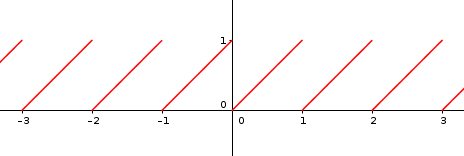
\includegraphics[width=0.5\textwidth]{immagini/esempio_serie_fourier.png}
\end{figure}
\\Osserviamo che nel caso la funzione presa in esame sia pari i coefficienti relativi alla parte dispari dello sviluppo, cioè i $b_n$, saranno tutti nulli, e viceversa, se la funzione è dispari, avremo che gli $a_n$, coefficienti relativi alla parte pari dello sviluppo, saranno tutti nulli.\\
Definiamo ora le somme parziali come la funzione:
$$S_N=a_0 + 2 \sum_{n=1} ^{N} \left[ a_n cos \left( \frac{2 \pi n}{b-a}x \right) + b_n sen \left( \frac{2 \pi n}{b-a}x \right) \right]$$
Quando si verifica che $S_N \to f$? Risostituendo le espressioni dei coefficienti $a_0$, $a_n$, $b_n$ e raccogliendo i fattori comuni, otteniamo otteniamo:
$$S_N=\frac{1}{b-a} \int_a ^b dy f(y) + 2 \sum_{n=1} ^{N} \left[ \frac{1}{b-a} \int_a ^b dy f(y) cos \left( \frac{2 \pi n}{b-a}y \right) cos \left( \frac{2 \pi n}{b-a}x \right) + \right.$$
$$\left. + \frac{1}{b-a} \int_a ^b dy f(y) sen \left( \frac{2 \pi n}{b-a}y \right) sen \left( \frac{2 \pi n}{b-a}x \right) \right]=$$
$$=\frac{1}{b-a} \int_a ^b dy f(y) \left\{ 1 + 2 \sum_{n=1} ^{N} \left[ cos \left( \frac{2 \pi n}{b-a}y \right) cos \left( \frac{2 \pi n}{b-a}x \right) + sen \left( \frac{2 \pi n}{b-a}y \right) sen \left( \frac{2 \pi n}{b-a}x \right) \right] \right\}=$$
$$=\frac{1}{b-a} \int_a ^b dy f(y) \left[ 1 + 2 \sum_{n=1} ^{N}  cos \left( \frac{2 \pi n}{b-a}(x-y) \right)\right] = \int_a ^b dy D_N(x-y) f(y)$$
dove abbiamo definito il \textbf{kernel di Dirichelet} $D_N$ come:
$$D_N=\frac{1}{b-a} \left[ 1 + 2 \sum_{n=1} ^{N}  cos \left( \frac{2 \pi n}{b-a}(x-y) \right)\right]$$
Una particolarità di tale operatore è che soddisfa l'equazione $ \int_a ^b dy D_N(x-y)=1$.
\subsection{Convergenza puntuale}
Se la funzione (sviluppata in serie di Fourier) $f$ è continua a meno di punti di discontinuità di prima specie tali per cui esistano le derivate da destra e da sinistra in tale punto, allora si verifica che $S_N \to f$ dove essa è continua, mentre converge nel ''punto medio'' dove $f$ presenta punti di discontinuità.\\
Se la funzione è molto liscia, allora i coefficienti della serie decresceranno molto rapidamente, altrimenti decrescono lentamente; questo ci porta a concludere c'è una relazione fra i coefficienti della serie di Fourier e le proprietà analitiche della funzione in esame.\\
Un'altra proprietà del kernel di Dirichelet è quella legata alla sua convergenza: infatti, per $N \to \infty$, abbiamo che il kernel $D_N(x-y) \to \delta (x-y)$ ripetuta infinite volte, poichè siamo in presenza di funzioni periodiche.\\
Per dimostrare che i coefficienti tendono ad annullarsi, scriviamo (detto $w=\frac{2 \pi}{b-a}$):
$$\int_a^b dx f(x) sen(wnx)=\int_a^b dx f(x) \left[\frac{d}{dx}\left(-\frac{cos(wnx)}{wn}\right)\right]=$$
$$=-\frac{f(x)cos(wnx)}{wn} + \int_a^b dx f'(x) \frac{cos(wnx)}{wn} \to 0 \text{ per } n \to \infty$$
Notiamo, infatti, che nel caso della funzione $f(x)cos(wnx)$, mediamo sia su valori positivi sia su valori negativi, e quindi quando $n$ è molto grande, abbiamo quasi il profilo della funzione ripetuto sia nella ''zona positiva'' sia nella ''zona negativa'' (sulle y). Per i $b_n$ procediamo in maniera simile.\\
A riguardo dell'annullamento dei coefficienti, risulta importante il seguente risultato dovuto a Riemann e Lebesgue:
\begin{teorema}
Se $f \in \cont^k([a;b])$, allora i coefficienti della serie di Fourier $a_n$, $b_n$ si annullano almeno come $\frac{1}{n^k}$ (per $n \to \infty$).
\end{teorema}
\subsection{Kernel di Fejer}
La teoria delle serie trigonometriche sviluppata da Lipot Fejer ci permette di provare la completezza degli spazi di Banach $\cont([- \pi ; \pi])$, $\L^1([- \pi ; \pi])$ e $\L^2 ([- \pi ; \pi])$. Questo ci assicura che qualsiasi funzione può essere approssimata con una combinazione finita di funzioni trigonometriche. \\
Una funzione $2 \pi$-periodica potrebbe ammettere serie di Fourier non convergente, e quindi non essere riprodotta come limite $N \to \infty$; a questo scopo, definiamo la somma di Fejer come la media aritmetica delle somme parziali, cioè:
$$\sigma _N= \frac{1}{N} \sum_{k=1} ^{N-1} S_k (x)= \int_{-\pi} ^{\pi} dt f(x+t) \Phi _N(t)$$
Dove $\Phi _N(t)$ è il \textbf{kernel di Fejer}, definito come:
$$\Phi _N(t)= \frac{1}{N} \sum_{k=1} ^{N-1} D_k (t)= \frac{1}{2 \pi} + \frac{1}{\pi} \sum_{k=1} ^{N-1} \left(1- \frac{k}{N} \right) cos(kt)= \frac{1}{2 \pi N} \frac{sen^2\left(\frac{Nt}{2}\right)}{sen^2\left(\frac{t}{2}\right)}$$
Tale scrittura ci permette di superare i problemi sopra esplicitati, e di approssimare la funzione come combinazione lineare di funzioni trigonometriche, senza ricorrere alla serie di Fourier.\\
Citiamo ora due teoremi, che non saranno qui dimostrati:
\begin{teorema}(Primo teorema di Fejer)\\
Se $f$ è reale continua e $2 \pi$-periodica, la successione di funzioni $\sigma _N$ converge uniformemente a $f$ in $\R$.
\end{teorema}
\begin{teorema}(Secondo teorema di Fejer)\\
Se $f \in \L^1([-\pi;\pi])$, la successione di somme di Fejer converge af $f$ in $\L^1([-\pi;\pi])$.
\end{teorema}
\section{Funzionali lineari e operatori aggiunti}
\begin{teorema}(Teorema di Riesz)\\
sia $F: \H \to \C$ un funzionale lineare continuo; allora esiste unico $x_F \in \H$ tale che $Fx=(x_F|x)$ $\forall x$ e $\|F\|=\|x_F\|$.
\end{teorema}
\begin{osservazione}
Per dimostrare questo teorema, esplicitiamo una proprietà del $\ker$ di un operatore. Sia $\hat{A} \in \mathcal{B}(\H)$, e sia $\H^*$ come definito in precedenza; allora l'insieme $\ker \hat{A}= \left\{ x: \, \hat{A}x=0 \right\}$ è chiuso. Infatti, presa una successione $x_n \in \ker \hat{A}$, e detto $x$ il limite di tale successione, per la continuità di $\hat{A}$ abbiamo che $\hat{A}x_n \to \hat{A}x$; ma allora, $\hat{A}x=0$, cioè $x \in \ker \hat{A}$.
\end{osservazione}
\begin{proof}
Nel caso banale, abbiamo che il $\ker F = \H$, cioè l'azione di $F$ su qualsiasi elemento $x$ è $Fx=0$; in questo caso, abbiamo che $x_F=0$.\\
Se invece il $\ker F$ non corrisponde con tutto lo spazio di Hilbert, possiamo scomporre $\H$ nella somma diretta di due sottospazi, $\ker F$ e $\ker F ^{\perp}$. Fissiamo ora un $y$ ortogonale all'insieme $\ker F$; per un $x$ generico, scegliamo $\lambda$ tale che $x+\lambda y \in \ker F$, cioè $F(x+\lambda y)=0$; risolvendo tale condizione, troviamo che $\lambda = -\frac{Fx}{Fy}$. La richiesta che $y$ non appartenga al $\ker F$ (è ortogonale ad esso) fa in modo che tale scrittura sia sempre ben posta. Possiamo quindi scrivere:
$$0=(y|x+\lambda y)=(y|x  -\frac{Fx}{Fy} y)=(y|x)  -\frac{Fx}{Fy} \|y\|^2 \implies Fx= \frac{Fy}{\|y\|^2} (y|x)= (x_F|x) \text{, dove } x_F=\frac{F^*y}{\|y\|^2} y$$
Per dimostrarne l'unicità, ipotizziamo che esistano due scritture equivalenti di questo tipo, $(x_F|x)$ e $(\tilde{x}|x)$, e che esse siano coincidenti $\forall x$; allora, abbiamo che:
$$0=(x_F|x) - (\tilde{x}|x)=(x_F - \tilde{x}|x) \, \, \forall x \implies x_F - \tilde{x}=0 \implies x_F = \tilde{x}$$
cioè la scrittura è unica.

Infine, dimostriamo l'identità delle norme:
$$|Fx|=|(x_P|x)| \leq \footnote{Applichiamo la disuguaglianza di Schwarz.} \|x_F\| \, \|x\| \implies \frac{|Fx|}{\|x\|} \leq \|x_F\| \implies \sup_{x, x \neq 0} \frac{|Fx|}{\|x\|} \leq \|x_F\|$$
quindi, preso $x=x_F$, abbiamo che $|Fx_F|=(x_F|x_F)=\|x_F\|^2$; dunque:
$$\frac{|Fx_F|}{\|x_F\|} =\frac{\|x_F\|^2}{\|x\|}= \|x_F\| \text{, cioè  } \|F\|=\|x_F\|$$
che è la tesi.
\end{proof}
Sia ora dato un operatore lineare limitato $\hat{A} \in \mathcal{B}(\H)$, il cui dominio è $\H$; il funzionale $(x|\hat{A} \cdot ): \H \to \C$ è lineare ed è limitato. Dimostriamone la limitatezza utilizzando il lemma di Schwatz:
$$|(x|\hat{A}y)|\leq \|x\| \, \|\hat{A}y\| \leq (\|x\| \, \|\hat{A}\|)\|y\|$$
dove la parentesi è una costante; abbiamo quindi dimostrato la limitatezza.
Possiamo applicare il teorema di Riesz al funzionale; abbiamo che $\forall x \in \H$ esiste un valore $\alpha_x$ tale che $(x|\hat{A}y)=(\alpha_x|y)$ $\forall y \in \H$. Preso un'altro valore $x'$, possiamo applicare lo stesso ragionamento, trovando un valore $\alpha_{x'}$; oltretutto, abbiamo che:
$$(x|\hat{A}y)+(x'|\hat{A}y)=(x+x'|\hat{A}y)=(\alpha_{x+x'}|\hat{A}y)$$
dove l'ultimo passaggio è possibile per il teorema si Riesz; però i primo membro è anche uguale a $(\alpha_x+\alpha_{x'}|\hat{A}y)$, cioè l'associazione $x \mapsto \alpha_x$ è lineare. Chiameremo tale associazione \textbf{operatore aggiunto}, e si indica come $\hat{A}^{\dagger} x= \alpha_x$.
\begin{teorema}
Sia $\hat{A} \in \mathcal{B}(\H)$; allora esiste $\hat{A}^{\dagger} \in \mathcal{B}(\H)$ tale che:
$$(x|\hat{A}y)=(\hat{A}^{\dagger}x|y)$$
$$\|\hat{A}\|=\|\hat{A}^{\dagger}\|$$
\end{teorema}
\begin{proof}
La linearità l'abbiamo dimostrata in precedenza; ci manca da dimostrarne la limitatezza:
$$\| \hat{A}^{\dagger} x \|^2=(\hat{A}^{\dagger}x|\hat{A}^{\dagger}x)=(x|\hat{A} \hat{A}^{\dagger} x) \leq  \|x\| \, \|\hat{A} \hat{A}^{\dagger} x \| \leq \|x\| \, \|\hat{A}\| \, \|\hat{A}^{\dagger} x \|$$
negli ultimi due passaggi sono stati sfruttati in ordine il lemma di Schwarz e la limitatezza di $\hat{A}^{\dagger}$;  allora abbiamo che:
$$\| \hat{A}^{\dagger} x \| \leq \|\hat{A}\| \, \|x \| \text{ } \forall x$$
e quindi $\hat{A}^{\dagger}$ è limitato, cioè $\hat{A}^{\dagger} \in \mathcal{B}(\H)$; oltretutto, abbiamo che $\|\hat{A}^{\dagger}\| \leq \|\hat{A}\|$.\\
Allo stesso modo, possiamo scrivere:
$$\| \hat{A}y \|^2=(\hat{A}y|\hat{A}y)=(\hat{A}^{\dagger} \hat{A} y|y) \leq  \|y\| \, \|\hat{A}^{\dagger} \hat{A} y \| \leq \|y\| \, \|\hat{A^{\dagger}}\| \, \|\hat{A} y \| \implies \|\hat{A}\| \leq \|\hat{A}^{\dagger}\|$$
Confrontando questo e il risultato precedente, otteniamo:
$$\|\hat{A}^{\dagger}\| \leq \|\hat{A}\| \leq \|\hat{A}^{\dagger}\| \implies \|\hat{A}\| = \|\hat{A}^{\dagger}\|$$
che è la nostra tesi.
\end{proof}
\clearpage
Lo spazio $\mathcal{B}(\H)$ è chiuso rispetto all'operazione $\dagger: \hat{A} \mapsto \hat{A}^{\dagger}$; le proprietà di tale operazione sono:
\begin{itemize}
\item $(\hat{A}^{\dagger})^{\dagger}= \hat{A}$
\item $( \lambda \hat{A})^{\dagger}= \overline{\lambda} \hat{A}^{\dagger}$
\item $(\hat{A} + \hat{B})^{\dagger}=\hat{A}^{\dagger} + \hat{B}^{\dagger}$
\item $(\hat{A} \hat{B})^{\dagger}=\hat{B}^{\dagger} \hat{A}^{\dagger}$
\end{itemize}
Sia dato un'operatore $\hat{A}$; esso è invertibile se è iniettivo, cioè se , qualora si abbia $\hat{A}x=\hat{A}x'$, allora $x=x'$. La linearità infatti implica che il $\ker$ dell'operatore si riduce al solo $0$; infatti, se risolviamo $\hat{A}(x-x')=0$, otteniamo che per iniettività si deve avere $x-x'=0$.\\
Cerchiamo ora una relazione fra un operatore e il suo aggiunto:
$$(Im \hat{A})^{\perp} = \left\{x \in \H : \, (x|\hat{A}y)=0 \, \forall y \in \H \right\} = \left\{x \in \H : \, (\hat{A} ^{\dagger}x|y)=0 \, \forall y \in \H \right\}=$$
$$=\left\{x \in \H : \hat{A}^{\dagger} x=0 \right\}= \ker \hat{A}^{\dagger}$$
Quindi $\ker \hat{A}^{\dagger}$ è un'insieme chiuso perchè è uguale a $(Im \hat{A})^{\perp}$, che è un'insieme chiuso. Possiamo quindi scrivere:
$$\H= \ker \hat{A} \oplus (\ker \hat{A})^{\perp}=(Im \hat{A})^{\perp} + \overline{Im \hat{A}^{\dagger}}$$
E, dato che l'uguaglianza vale termine a termine, possiamo sommare un termine di $\ker$ e un termine di $Im$ (non a caso); questo è importante quando dobbiamo risolvere un'equazione del tipo $\hat{A}x=y$: infatti, se siamo in uno spazio finito-dimensionale, abbiamo delle condizioni che devono essere soddisfatte per poter discutere la risolubilità (ad esempio, l'invertibilità della matrice). Se invece siamo in uno spazio $\infty$-dimensionale, ci chiediamo se $y \in Im \hat{A}$.\footnote{Alternativamente, possiamo utilizzare il metodo di Fredom, secondo il quale se $\ker \hat{A}^{\dagger}=0$ allora esiste una soluzione.}
\begin{definizione}
Un'operatore $\hat{A} \in \mathcal{B}(\H)$ si dice \textbf{autoaggiunto} se $\hat{A}=\hat{A}^{\dagger}$, cioè se vale che:
$$(\hat{A}x|y)=(x|\hat{A}^{\dagger}y) \, \, \forall x, y \in \H$$
\end{definizione}
Un esempio di operatore autoaggiunto che abbiamo già visto in precedenza è il proiettore ortogonale; infatti avevamo visto che fra le proprietà di tale operatore c'era proprio l'essere autoaggiunto; inoltre, detto $Im \hat{P}$ sottospazio di proiezione, abbiamo che nel caso in cui tale sottospazio abbia dimensione finita, vale che $\tr \hat{P}=\dim Im \hat{P}$.
\begin{definizione}
Lo scalare $\lambda \in \C$ si dice \textbf{autovalore proprio} dell'operatore $\hat{A}$ se esiste un elemento $u \in \H$ tale che $\hat{A} u = \lambda u$. Nel caso in cui $\hat{A}$ sia autoaggiunto, allora $\lambda$ è reale.\\
L'insieme degli  autovalori di un operatore è detto \textbf{spettro puntuale} dell'operatore e si indica con $\sigma_P (\hat{A})$.
\end{definizione}
Siano $\lambda , \mu \in \sigma_P (\hat{A})$, cioè siano essi due autovalori dell'operatore $\hat{A}$; se $\lambda \neq \mu$, allora si ha che $(u|v)=0$, dove $u$ e $v$ sono gli autovalori relativi rispettivamente a $\lambda$ e $\mu$. Questo ci dive che possiamo scomporre uno spazio di Hilbert come somma ortogonale  dello spazio generato dagli autovettori (che, come appena visto, sono ortogonali fra loro) e il suo spazio ortogale:
$$\H=\H_P \oplus \H_P ^{\perp}=\H_P \oplus \H_C$$
Nel caso dei proiettori, abbiamo $\H_C=\varnothing$.
\section{Operatori unitari}
Definiamo l'operatore unitario $\hat{U}$ come quell'operatore tale che sia una biezione e che rispetti l'uguaglianza fra norme:
$$\|\hat{U}x\|=\|x\| \, \, \forall x$$
Altre proprietà degli operatori unitari sono:
\begin{itemize}
\item Il prodotto di operatori unitari è unitario.
\item $\ker \hat{U}= \{0\}$
\item Vale che $(\hat{U}x|\hat{U}y)=(x|y)$; da questa proprietà ricaviamo che un'operatore unitario e il suo aggiunto commutano; infatti, per la definizione di aggiunto possiamo scrivere:
$$(\hat{U}x|\hat{U}y)=(\hat{U}^{\dagger} \hat{U} x|y)$$
e, sottraendo il secondo membro dell'equazione di partenza, otteniamo:
$$([\hat{U}^{\dagger} \hat{U} - \mathbb{I}]x|y)=0 \implies \hat{U}^{\dagger} \hat{U} = \mathbb{I}$$
e alla stessa maniera ricaviamo $ \hat{U} \hat{U}^{\dagger} = \mathbb{I}$; mettendo insieme le due condizioni (che valgono $\forall x,y$), si ottiene che il commutatore fra l'operatore e il suo aggiunto è nullo, cioè commutano.
\item Gli autovalori stanno tutti sulla circonferenza unitaria; infatti, detto $\lambda$ autovalore relativo all'autovettore $x$, per l'identità delle norme abbiamo:
$$\|x\|=\|\hat{U}x\|=\|\lambda x\|=|\lambda| \, \|x\| \implies |\lambda|=1$$
\end{itemize}
Abbiamo visto che, dato un operatore $\hat{A} \in \mathcal{B}(\H)$, possiamo sempre ricavarne l'esponenziale $e^{z \hat{A}}$, con $z \in \C$ che è a sua volta un'operatore limitato. Sviluppando in serie, possiamo definire la funzione $S_N(z)$, cioè le somme parziali dello sviluppo in serie nella variabile $z$. saranno della forma:
$$S_N(z)= \sum_{k=0} ^N \frac{(z \hat{A})^k}{k!} \to e^{z \hat{A}} \text{ per } N \to \infty$$
A questo punto, possiamo dimostrare che per gli operatori vale che $e^{(z_1+z_2) \hat{A}}=e^{z_1 \hat{A}} e^{z_2 \hat{A}}$ utilizzando le somme parziali; scriviamo:
$$S_N(z_1+z_2)=\sum_{k=0} ^N \frac{[(z_1+z_2) \hat{A}]^k}{k!} = \footnote{Sfruttiamo lo sviluppo tramite binomio di Newton.} \sum_{k=0} ^N \frac{ \hat{A}^k}{k!} \sum_{j=0} ^N \frac{k!}{j! (k-j)!} z_1^j z_2 ^{k-j}=$$
$$=\sum_{j=0} ^N \frac{z_1^j}{j!} \sum_{k=j} ^N \frac{z_2 ^{k-j}}{(k-j)!} \hat{A}^k =\sum_{j=0} ^N \frac{z_1^j}{j!} \sum_{k=0} ^{N-j} \frac{z_2 ^k}{k!} \hat{A}^{k+j}= \sum_{j=0} ^N \frac{(z_1 \hat{A})^j}{j!} \sum_{k=0} ^{N-j} \frac{(z_2 \hat{A})^k}{k!} = S_N(z_1) S_N(z_2)$$
e, nel limite di $N \to \infty$, abbiamo la tesi.\\
Nel caso in cui $\hat{A}$ sia autoaggiunto, possiamo definire l'esponenziale $e^{it\hat{A}}$, con $t \in \R$; tale operatore esponenziale è un'operatore unitario, e quindi commuta con il suo aggiunto. Infatti, detto $\hat{U}$ l'operatore esponenziale, si ha:
$$\hat{U}^{\dagger} (t)= \left(e^{it\hat{A}}\right)^{\dagger}=e^{-it\hat{A}^{\dagger}}=\hat{U}(-t)$$
e dunque, il prodotto $\hat{U}^{\dagger} \hat{U}$ dà l'identità, e la stessa cosa scambiando i fattori. L'operatore $i \hat{A}$ (dove $\hat{A}$ e come definito in precedenza) è detto \textbf{operatore antiautoaggiunto}, poichè il suo aggiunto è il suo opposto, cioè è autoaggiunto a meno di un segno.\\
L'insieme di operatori $\hat{U} (t)$ è un gruppo a un parametro (che è $t$) di operatori unitari, con continuità forte nell'origine, cioè:
$$\lim_{t \to 0} \| \hat{U}(t) x - x \|_{\H}=0$$
La matrice che genera tale gruppo di operatori è detta \textbf{generatore del gruppo a un parametro}.
\begin{teorema}
Sia $\hat{U} (t)$ un gruppo a un parametro di operatori unitari fortemente continuo. Allora esiste un'operatore autoaggiunto $\hat{H}$, in generale non limitato, tale che:
$$\hat{U}(t)=e^{-it \hat{H}}$$
Si ha inoltre che il dominio di tale operatore è:
$$\mathcal{D} (\hat{H})= \left\{x \in \H \text{ : } \exists \lim_{t \to 0} \frac{e^{-it\hat{H}} x - x}{-it} \right\}$$
\end{teorema}
Sia dato l'operatore $\hat{A}$ a valori in $\H$; abbiamo definito l'operatore aggiunto $\hat{A}^{\dagger}$ come quell'operatore tale per cui $(x|\hat{A}y)=(\hat{A}^{\dagger} x|y)$ $\forall x \in \mathcal{D}({\hat{A}^{\dagger}})$, $\forall y \in \mathcal{D}({\hat{A}})$. In quale occasione possiamo trovare l'operatore aggiunto? Solo nel caso in cui il dominio di tale operatore sia della forma:
$$\mathcal{D}({\hat{A}^{\dagger}})=\left\{ x \in \H \text{ : } \forall y \in \mathcal{D}({\hat{A}}) \, \exists ! \tilde{x} \text{ : } (x|\hat{A}y)=(\tilde{x}|y) \right\}$$
Una volta caratterizzata in questa maniera il dominio, diremo che $\tilde{x}=\hat{A}^{\dagger} x$.\\
Ragioniamo sulla richiesta di unicità: supponiamo che, fissato $x$, esistano $\tilde{x}$ e $x'$ tali che $(\tilde{x}|y)=(x|\hat{A}y)$ e $(x'|y)=(x|\hat{A}y)$ $\forall y \in \mathcal{D}(\hat{A})$; sottraendo membro a membro le due uguaglianze, otteniamo:
$$(\tilde{x} - x'|y)=0 \, \, \forall y \in \mathcal{D}(\hat{A})$$
cioè $(\tilde{x}-x') \in (\mathcal{D}(\hat{A}))^{\perp}$. La richiesta di unicità ci permette di concludere che $\tilde{x}=x'$, cioè che $(\mathcal{D}(\hat{A}))^{\perp} = \left\{0\right\}$, cioè che $\overline{\mathcal{D}(\hat{A})}= \H$. Quindi l'operatore deve essere \textbf{densamente definito}, cioè per ogni elemento dello spazio di Hilbert è limite di una successione di elementi di $\hat{A}$.\\
Adesso dimostriamo che, dato $\hat{A} \in \mathcal{B}(\H)$,  vale la relazione $\| \hat{A}^{\dagger} \hat{A} \|= \| \hat{A} \|^2$; utilizzando la proprietà della norma tale per cui $\| \hat{A} \hat{B} \| \leq \| \hat{A} \| \, \| \hat{B} \|$, scriviamo:
$$\| \hat{A}^{\dagger} \hat{A} \| \leq \|\hat{A}^{\dagger}\| \, \|\hat{A}\|= \|\hat{A}\| \, \|\hat{A}\| = \|\hat{A}\|^2$$
Inoltre, sfruttando la disuguaglianza di Schwarz, possiamo scrivere:
$$\| \hat{A}x\|^2=(\hat{A}x|\hat{A}x)=(\hat{A}^{\dagger} \hat{A}x|x) \leq \| \hat{A}^{\dagger} \hat{A}\| \, \|x\|$$
e, prendendo il sup, otteniamo:
$$\|\hat{A}\| = \sup_{x \neq 0} \frac{\|\hat{A}x\|}{\|x\|} \leq \|\hat{A}^{\dagger} \hat{A}\|^{\frac{1}{2}}$$
unendo le due condizioni, dimostriamo la tesi.\\
Possiamo definire la norma di un'operatore in altro modo:
$$\|\hat{A}\|=\sup_{\|x\|=1} |(x|\hat{A}x)|$$
\clearpage
\section{Spazi di Schwarz}
A Schwarz si deve l'introduzione di due spazi: lo \textbf{spazio di Schwarz}, cioè lo spazio delle funzioni $\cont^{\infty}$ a decrescenza rapida, indicato nella forma $\S(\R)$, e lo spazio $\mathscr{D}(\R)$, cioè lo spazio delle funzioni $\cont^{\infty}$ a supporto compatto; notiamo che lo spazio $\mathscr{D}$ è contenuto nello spazio $\S$.\\
Inoltre, a partire da questi due spazi, possiamo definirne altri due: lo spazio delle \textbf{distribuzioni temperate} $\S'(\R)$ e lo spazio delle distribuzioni $\mathscr{D}'(\R)$; in questo caso, invece, abbiamo che lo spazio $\S'$ è contenuto nello spazio $\mathscr{D}'$.\\
Una proprietà fondamentale dello spazio di Schwarz $\S$ è quella di essere invariante per la trasformata di Forier, cioè tale operatore, che definiremo poco più avanti, manda $\S$ in se stesso; inoltre, lo spazio $\S$ è sottoinsieme dello spazio $\L^2$ e la sua chiusura (nella norma di $\L^2$) è proprio lo spazio $\L^2$.\\
Il contributo di Gelfrand è molto importante nello studio di questi spazi; infatti egli introdusse le cosìddette \textbf{funzioni generalizzate} (come ad esempio la delta di Dirach), che permettono di trattare distribuzioni con strumenti pensati per le funzioni.
\\
\\
Prima però di passare allo studio delle distribuzioni, trattiamo più approfonditamente  i concetti appena introdotti; prima di tutto, diamo una definizone di \textbf{decrescenza rapida}:
\begin{definizione}
Una funzione $f$ si dice a \textbf{decrescenza rapida} se, $\forall m,n \geq 0$, esiste finita la quantità:
$$\|f\|_{m,n} = \sup_{x \in \R} |x^m (D^n f)(x)|$$
dove abbiamo indicato con $D^n$ l'operazione di derivata $n$-esima, cioè $D^n=\frac{d^n}{dx^n}$.
\end{definizione}
La decrescenza rapida mi permette quindi di fare in modo che tale quantità non esploda ad infinito qualsiasi valore io scelga per le costanti $n$ e $m$. Funzioni di questo tipo sono per esempio $e^{-x^2}$ e i polinomi di Hermite. Notiamo che l'operazione $\| \cdot \|_{m,n}$ definisce una \textbf{famiglia di seminorme}, poichè rispetta le seguenti proprietà:
\begin{itemize}
\item $\| \phi_1 + \phi_2 \|_{m,n} \leq \| \phi_1\|_{m,n} + \|\phi_2\|_{m,n}$
\item $\| \lambda \phi \|_{m,n} = | \lambda | \, \| \phi \|_{m,n}$
\end{itemize}
Lo spazio $\cont(\R)$ è lo spazio delle funzioni continue che si annullano ad $\infty$; esso è uno spazio di Banach, dove la norma è definita come:
$$\|f\|= \sup_x |f(x)|$$
Si verifica che $\S \subset \cont$. Un'altra inclusione importante per lo studio dello spazio di Schwarz è $\S \subset \L^1$; detto ciò, presa una funzione $\phi \in \S$, abbiamo che:
$$\| \phi \|_1 = \int_{- \infty} ^{+\infty} dx | \phi (x) |= \int_{- \infty} ^{+\infty} dx | \phi (x) | \frac{1+x^2}{1+x^2} \leq \sup_x | \phi (x) (1+x^2)| \int_{- \infty} ^{+\infty} dx \frac{1}{1+x^2}=$$
$$=\sup_x | \phi (x) (1+x^2)| \pi  \leq \left( \| \phi \|_{0,0} + \| \phi \|_{2,0} \right) \pi$$
Allo stesso modo, possiamo dimostrare che $\S \subset \L^p$:
$$\| \phi \|_p ^p = \int_{- \infty} ^{+\infty} dx | \phi (x) |^p = \int_{- \infty} ^{+\infty} dx | \phi (x) |^{p-1} | \phi (x) | \leq \| \phi \|_{0,0} \int_{- \infty} ^{+\infty} dx | \phi (x) |^{p-1} \leq \dots \leq \| \phi \|_{0,0} ^{p-1} \, \| \phi \|_1$$
Definiamo ora la convergenza in $\S(\R)$:
\begin{definizione}
Una successione $\phi_r$ converge a $\phi$ in $\S$ se $\| \phi_r - \phi \|_{m,n} \to 0$ $\forall m,n$.
\end{definizione}
\clearpage
Per far sì che lo spazio sia completo, ci rimane da introdurre la nozione di successione di Cauchy:
\begin{definizione}
Una successione è di Cauchy se
$$\forall \epsilon >0 \, \, \exists N_{\epsilon , m,n} \text{ : }\|\phi_r -\phi_s \|_{m,n} < \epsilon \, \, \forall r,s > N_{\epsilon , m,n} \text{, con }m,n=0,1 \dots$$
\end{definizione}
Ora quindi possiamo enunciare il seguente teorema:
\begin{teorema}
Lo spazio $\S(\R)$ è completo.
\end{teorema}
Quando sono completi, questi spazi non sono più detti spazi di Banach, ma \textbf{spazi di Frechet}.
Nella definizione di successione di Cauchy, riscriviamo la norma come da definizione, cioè $\| \phi_r - \phi_s \| = \sup_{x \in \R} |x^m D^n (\phi_r - \phi_s)|$. Notiamo che, nel caso in cui $m=n=0$, allora la convergenza in $\S$ coincide con la convergenza per funzioni reali a variabili reali; quindi  $\phi_r$ è una successione di Cauchy in $\cont(\R)$, cioè converge alla funzione $\psi_{0,0} \in \cont(\R)$. Generalizzando per ogni coppia di $m,n$, abbiamo che $x^m D^n \phi_r$ è una successione di Cauchy nello spazio $\cont(\R)$, cioè converge alla funzione $\psi_{m,n} \in \cont(\R)$; si dimostra che $\psi_{m,n}=x^m D^n \psi_{0,0}$.
\\
Passiamo ora a trattare gli operatori sullo spazio $\S$:
\begin{itemize}
\item \textbf{Operatore di moltiplicazione $\hat{Q}$}: tale operatore è definito in $\S$ a valori in $\S$ ed è continuo; la sua azione sulla funzione $\phi \in \S$ è:
$$(\hat{Q} \phi)(x)=x \phi(x)$$
Dimostriamo che la norma in $\S$ di tale operatore è finita, cioè che $\hat{H}\phi \in \S$:
$$\sup_x |x^m D^n (\hat{Q} \phi)(x)|=\sup_x |x^m D^n (x \phi)|= \sup_x |x^m D^{n-1} \phi + x^{m+1} D^n \phi| \leq$$
$$\leq \sup_x |x^m D^{n-1} \phi| + \sup_x |x^{m+1} D^n \phi|= \| \phi \|_{m,n-1} + \| \phi \|_{m+1,n}$$
Quindi, poichè le due seminorme sono quantità finte, abbiamo che anche la seminorma dell'operatore è finita e dunque $\hat{Q} \phi \in \S$. Dimostriamo ora la continuità dell'operatore; data la linearità di $\hat{Q}$, ci basta dimostrarne la continuità nell'origine. Data una successione $\phi_r$ che converge a $0$ in $\S$ per $r \to \infty$, abbiamo che $\hat{Q} \phi_r \to 0$ in $\S$; infatti, passando alle seminorme, abbiamo che la seminorma $\| \hat{Q} \phi \|_{m,n}$ è minorata dalla somma di due seminorme della funzione $\phi_r$ e, dato che la condizione di annullamento di $\phi_r$ equivale a dire che $\| \phi_r \|_{m,n} \to 0$ $\forall m,n$, abbiamo che le due seminorme tendono ad annullarsi nel limite per $r \to \infty$, e dunque anche l'operatore applicato a $\phi_r$ tende a $0$.
\item \textbf{Operatore $\hat{P}$}: anch'esso definito in $\S$ a valori in $\S$ e continuo, ha azione descritta da:
$$\hat{P} \phi = -i D \phi$$
dove ricordiamo che la $D$ indica l'operazione di derivazione; l'operatore risulta invertibile, poichè si ha che $\ker \hat{P} = \left\{ 0 \right\}$: infatti la derivata di $\phi$ si annulla solo nel caso in cui $\phi$ sia costante e, dato che siamo nello spazio $\S$, non può che essere $\phi = 0$.
\end{itemize}
\section{La trasformata di Fourier}
Definiamo su $\S$ due operatori lineari:
$$\left( \F \phi \right) (k) = \int_{-\infty} ^{+\infty} \frac{dx}{\sqrt{2 \pi}} e^{-ikx} \phi (x)$$
$$\left( \F^{-1} \phi \right) (k) = \int_{-\infty} ^{+\infty} \frac{dx}{\sqrt{2 \pi}} e^{ikx} \phi (x)=\left( \F \phi \right) (-k)$$
dove $k$ è un parametro definito in $\R$.

La prima è detta \textbf{trasformata di Fourier}, la seconda \textbf{antitrasformata di Fourier}. Osserviamo che entrambe sono definite in $\S$ a valori in $\S$ e $\F \phi \in \cont^{\infty}$ (possiamo portare la derivata all'interno dell'integrale e otteniamo che $x^n \phi \in \S$); verifichiamo quindi che $\| \F \phi \|_{m,n} < \infty$ $\forall m,n$:
$$x^m D_x ^n \left( \F \phi \right) (x) = x^m \int_{-\infty} ^{+\infty} \frac{dk}{\sqrt{2 \pi}} \left( D_x ^n e^{-ikx} \right) \phi (k) = x^m \int_{-\infty} ^{+\infty} \frac{dk}{\sqrt{2 \pi}} (-ik)^n e^{-ikx} \phi (k) =\footnote{Possiamo portare dentro l'integrale $x^m$, poichè stiamo integrando su $k$, e lo vediamo come derivata $m$-esima (rispetto a $k$) dell'esponenziale.}$$
$$= \int_{-\infty} ^{+\infty} \frac{dk}{\sqrt{2 \pi}} \frac{(-ik)^n}{(-i)^m} \left( D^m _k e^{-ikx} \right) \phi (k) =\footnote{Integramo per parti $m$-volte; possiamo ignorare i termini di bordo, poichè la funzione $\phi$ è a decrescenza rapida, e quindi batte qualsiasi potenza.} (-1)^m (-i)^{n-m} \int_{-\infty} ^{+\infty} \frac{dk}{\sqrt{2 \pi}} e^{-ikx} D_k ^m \left( k^n \phi (k) \right)$$
L'operazione di derivazione ci darà al più $m+1$ termini del tipo $x^{\alpha} D^{\beta} \phi$, con $\alpha = n,n-1, \dots ,n-m$ e $\beta=0,1, \dots ,m$; quindi possiamo scrivere:
$$\left|x^m \left(D^n \F \phi \right) (x) \right| \leq \sum_{\alpha, \beta} \int_{-\infty} ^{+\infty} \frac{dk}{\sqrt{2 \pi}} | k^{\alpha} \phi^{\beta} (k) | \frac{1+k^2}{1+k^2} = \pi \Sigma_N [\phi]$$
dove il termine $ \Sigma_N [\phi]$ indica una somma finita di seminorme di $\phi$; quindi abbiamo che la quantità $\| \F \phi \|_{m,n}$ è finita per ogni coppia di valori $m,n$.
\\
\\
Abbiamo detto che la trasformata di fourier è un'operatore lineare che manda $\S$ in $\S$; si ha inoltre che $\F$ è un'operatore continuo, cioè se applicato ad una successione convergente restituisce una successione convergente. Anche in questo caso come per l'operatore di moltiplicazione ci basta  dimostrare la continuità nell'origine, cioè dimostrare la seguente implicazione in $\S$:
$$\phi_r \to 0 \implies \| \F \phi_r \| \to 0$$
Tutte le proprietà enunciate per la trasformata di Fourier valgono anche per l'antitrasformata; adesso, mostriamo che effettivamente i due operatori, come suggerisce la scrittura, sono uno l'inverso dell'altro:
\begin{teorema}(Teorema di inversione per la trasformata di Fourier)\\
L'inverso della trasformata di Fourier $\F$ è l'antitrasformata $\F^{-1}$, cioè $\F \o \F^{-1}= \F^{-1} \o \F= \mathbb{I}$; in forma integrale:
$$ \int_{-\infty} ^{+\infty} \frac{dk}{\sqrt{2 \pi}} e^{-ikx}\left( \F \phi \right) (k) =  \int_{-\infty} ^{+\infty} \frac{dk}{\sqrt{2 \pi}} e^{ikx} \left( \F^{-1} \phi \right) (k) = \phi(x)$$
\end{teorema}
Per dimostrare il teorema, introduciamo prima un lemma che ci sarà molto utile:
\begin{lemma}
sia definito l'operatore $\hat{E_{\epsilon}} (x)= e^{- \epsilon x^2}$; allora abbiamo che $\hat{E_{\epsilon}} \phi \in \S$ e il suo limite in $\S$ per $\epsilon \to 0^+$ è $\phi$.
\end{lemma}
\begin{proof}
Dobbiamo dimostrare che la norma della funzione è finita, cioè che $\sup_x |x^m D^n (e^{- \epsilon x^2} \phi (x))| < \infty$ $\forall m,n$; equivalentemente, possiamo dimostrare che $\sup_x |x^m D^n (e^{- \epsilon x^2} \phi (x)- \phi(x))| \to 0$ per $\epsilon \to 0$ $\forall m,n$.
$$\lim_{\epsilon \to 0} \| \hat{E_{\epsilon}} \phi - \phi \|_{m,n}= \lim_{\epsilon \to 0} \sup_x \left[ (1-e^{- \epsilon x^2})|x^m D^n  \phi (x)|\right]$$
dove possiamo maggiorare il coefficiente $(1-e^{- \epsilon x^2})$ nella seguente maniera:
$$1-e^{- \epsilon x^2} \left\{\begin{matrix} =0 & x=0 \\ \leq 2 \epsilon x^2 & x \neq 0 \end{matrix} \right.$$
e quindi nel limite di $\epsilon \to 0$ la norma si annulla sempre.
\end{proof}
Dunque, se $\hat{E_{\epsilon}} \phi$ tende a $0$ nel limite per $\epsilon \to 0$, allora, per la continuità della trasformata e dell'antitrasformata, abbiamo che $\F^{-1} \left(\hat{E_{\epsilon}}\left(\F \phi \right) \right) \to \F^{-1} \F \phi$ in $\S$; possiamo utilizzare questa proprietà per dimostrare che $\F^{-1} \F \phi = \phi$ o, equivalentemente, che $\F^{-1} \F \phi - \phi = 0$.\\
Abbiamo che:
$$\F ^{-1} \hat{E_{\epsilon}} \F \phi = \int_{-\infty} ^{+\infty} \frac{dk}{\sqrt{2 \pi}} e^{ikx} e^{-\epsilon k^2} \int_{-\infty} ^{+\infty} \frac{dy}{\sqrt{2 \pi}} e^{-iky} \phi (y)$$
Cambiando ordine di integrazione, otteniamo:
$$\int_{-\infty} ^{+\infty} dy \phi (y) \int_{-\infty} ^{+\infty} \frac{dk}{2 \pi} e^{-ik(y-x) -\epsilon k^2} = \int_{-\infty} ^{+\infty} dy \phi (y) \int_{-\infty} ^{+\infty} \frac{dk}{2 \pi} e^{- \epsilon \left( k + \frac{y-x}{2 \epsilon} \right)^2  -\frac{(y-x)^2}{4 \epsilon}} =$$
$$= \int_{-\infty} ^{+\infty} dy \phi (y) e^{ -\frac{(y-x)^2}{4 \epsilon}} \frac{1}{2 \pi} \frac{\sqrt{\pi}}{\sqrt{\epsilon}} =  \int_{-\infty} ^{+\infty} dy \phi (y) k_{\epsilon} (x-y)$$
Dove abbiamo abbiamo definito il kernel dell'equazione del calore:
$$ k_{\epsilon} (x-y) = \frac{1}{2 \sqrt{ \pi \epsilon}} e^{ -\frac{(y-x)^2}{4 \epsilon}}$$
Notiamo che, per $\epsilon \to 0$, tale kernel tende alla $\delta (x-y)$; inoltre, abbiamo che il kernel è normalizzato, cioè $ \int_{-\infty} ^{+\infty} dx k_{\epsilon} (x)=1$. Ora, ci rimane da dimostrare che:
$$\lim_{\epsilon \to 0}  \int_{-\infty} ^{+\infty} dy \left( \phi (y) - \phi (x) \right) k_{\epsilon} (x-y)=0$$
Per farlo, prendiamo il modulo e maggioriamo:
$$|\int_{-\infty} ^{+\infty} dy \left( \phi (y) - \phi (x) \right) k_{\epsilon} (x-y)| \leq \int_{-\infty} ^{+\infty} dy | \phi (y) - \phi (x) | \, |k_{\epsilon} (x-y)| \leq$$
$$ \leq \int_{-\infty} ^{+\infty} dy |\phi' (\xi_{x,y})| \, |x-y| \frac{1}{2 \sqrt{ \pi \epsilon}} e^{ -\frac{(y-x)^2}{4 \epsilon}} \leq \footnote{Eseguiamo un cambio di variabili $z=x-y$.} \sup_z |\phi' (\xi_{x,y})| \int_{-\infty} ^{+\infty} dz |z|  \frac{1}{2 \sqrt{ \pi \epsilon}} e^{ -\frac{(y-x)^2}{4 \epsilon}}$$
Dunque, abbiamo che:
$$|\F^{-1} \hat{E_{\epsilon}} \F \phi - \phi| \leq 2 \| \phi \|_{0,1} \int_0 ^{+\infty} dz \frac{z}{2 \sqrt{ \pi \epsilon}} e^{ -\frac{(y-x)^2}{4 \epsilon}}= \footnote{Altro cambio di variabili; in questo caso, scriviamo $z= \sqrt{\epsilon} t$.} 2 \| \phi \|_{0,1}  \frac{\sqrt{\epsilon}}{2 \sqrt{\pi}} \int_0 ^{+\infty} dt \, t \,  e^{ -\frac{t^2}{4}}$$
che, nel limite per $\epsilon \to 0$, tende a 0.
\subsection{Proprietà della trasformata di Fourier}
Abbiamo introdotto la trasformata $\F$ e l'antitrasformata $\F^{-1}$ come operatori definiti in $\S$ a valori in $\S$; oltretutto, tramite il teorema di inversione, abbiamo visto che $\F \o \F^{-1}=\mathbb{I}$. Altre proprietà utili di quest'operatore sono:
\begin{itemize}
\item L'operatore $\F$ elevato al quadrato si comporta come l'operatore parità, cioè si ha che $(\F^2 \phi )(x)=\phi(-x)$; infatti, per dimostrarlo basta dire che $(\F^2 \phi )(x)=(\F^{-1} \F \phi)(-x)= (\mathbb{I} \phi)(-x)= \phi(-x)$
\item Valgono le seguenti identità fra operatori:
$$\F \hat{Q}=-\hat{P}\F$$
$$\hat{Q} \F= \F \hat{P}$$
Dimostriamo la seconda; la prima si dimostra in modo analogo. Vale che:
$$(\hat{Q} \F \phi)(x)=x(\F \phi)(x) = x \int_{-\infty}^{+\infty} \frac{dk}{\sqrt{2 \pi}}e^{-ikx} \phi(k)=  \int_{-\infty}^{+\infty} \frac{dk}{\sqrt{2 \pi}} i \left( \frac{d}{dk} e^{-ikx} \right) \phi(k)$$
a questo punto, integriamo per parti; i termini di bordo si annullano, e ci rimane:
$$(\hat{Q} \F \phi)(x)=-i \int_{-\infty}^{+\infty} \frac{dk}{\sqrt{2 \pi}}e^{-ikx} \phi'(k)=(\F (-i \phi'))(x)=(\F \hat{P} \phi)(x)$$
\item $\left[ \hat{Q}^2 + \hat{P}^2 , \F \right]=0$
\item $(\F u_n)(x)= (-i)^n u_n (x)$, cioè la trasformata di Fourier di una funzione di Hermite è una funzione di Hermite; dunque le funzioni di Hermite sono autovettori della trasformata di Fourier relativi agli autovalori $(-i)^n$. %Per dimostrare questo fatto, si trova la funzione generatrice degli $u_n$, che sarà nella forma:
%$$h(t,x)=\sum_{n=0}^{\infty} \frac{t^n}{\sqrt{n!}} \frac{1}{\sqrt{n! 2^n \sqrt{\pi}}} e^{\frac{x^2}{2}} H_n(x)$$
%notiamo che 
\item $(\phi|\F \psi)=(\F^{-1} \phi|\phi)$; se sosituiamo la $\phi$ con $\F \xi$, otteniamo che:
$$(\F \xi | \F \psi )=(\xi|\psi) \text{ } \forall \phi, \psi, \xi \in \S(\R)$$
cioè abbiamo che la trasformata di Fourier si comporta come un operatore unitario. Dimostriamo questa proprietà:
$$(\phi | \F \psi)= \int_{-\infty} ^{+\infty} dx \overline{\phi (x)} \left(\F \psi \right) (x)= \int_{-\infty} ^{+\infty} dx \overline{\phi (x)}  \int_{-\infty} ^{+\infty} \frac{dk}{\sqrt{2 \pi}} e^{-ikx} \psi(k)=$$
$$=\int_{-\infty} ^{+\infty} \frac{dk}{\sqrt{2 \pi}} \left[ \int_{-\infty} ^{+\infty} dx \overline{\phi (x)} \, \overline{e^{ikx}}  \right] \psi(k) =  \int_{-\infty} ^{+\infty} dk \overline{\left( \F^{-1} \phi \right) (k)} \psi(k)=(\F^{-1} \phi | \psi)$$
Inoltre, grazie al teorema dell'inversione, possiamo scrivere:
$$\phi(x)=\left(\F^{-1} \F \phi \right) (x) = \int_{-\infty} ^{+\infty} dk \frac{e^{ikx}}{\sqrt{2 \pi}} \left(\F \phi \right) (x) =  \int_{-\infty} ^{+\infty} dk \frac{e^{ikx}}{\sqrt{2 \pi}} \tilde{\phi} (k)$$
dove abbiamo che $\tilde{\phi} (k)=  \int_{-\infty} ^{+\infty} dx \frac{e^{-ikx}}{\sqrt{2 \pi}} \phi(x)$.
\item Possiamo dimostrare la completezza della base dei polinomi di Hermite in $\L^2 (\R)$; infatti:
$$(u_n|u_m)= \delta_{nm} \text{, con la normalizzazione data da }\frac{1}{\sqrt{n! 2^n \sqrt{\pi}}}$$
Verifichiamo ora che $(u_n|f)=0 \, \forall n \implies f=0$ q.o.; la condizione è equivalente a richiedere che $(H_t|f)=0 \, \forall t$, dove ricordiamo che $H_t$ è la funzione generatrice dei polinomi di Hermite. Svolgendo i calcoli, otteniamo:
$$ \int_{-\infty} ^{+\infty} \frac{dx }{\sqrt{2 \pi}} e^{-ikx - \frac{1}{2} x^2} f(x)=0 \, \, \forall k$$
attraverso la disuguaglianza di Schwarz è possibile verificare che $f \, e^{-\frac{1}{2}x^2} \in \L^1 (\R)$, dunque possiamo farne la trasformata di Fourier; dato che $\ker \F = \{0\}$ in $\L^1 (\R)$, deve essere che $f \, e^{-\frac{1}{2}x^2} = 0$ q.o. e quindi la base dei polinomi di Hermite è completa.
\end{itemize}

\subsection{Il prodotto di convoluzione}
Ci proponiamo di rappresentare attraverso una funzione $g(x)$ l'integrale $\int_{-\infty} ^{+\infty} dy \, k(x-y) \, f(y)$, dove $x$ è assegnato; a questo proposito, negli spazi $\S$ viene introdotto il \textbf{prodotto di convoluzione} fra due elementi di $\S$, definito come:
$$\left(\phi \ast \psi \right) (x) = \int_{-\infty} ^{+\infty} dy \, \phi(x-y) \, \psi(y)$$
Le proprietà di tale operazione sono:
\begin{itemize}
\item $\phi \ast \psi = \psi \ast \phi$, cioè è commutativo.
\item Gode della proprietà distributiva, cioè $\phi \ast (\psi_1 + \psi_2)=(\phi \ast \psi_1) + (\phi \ast \psi_2)$.
\item Se $\phi, \psi \in \S$, allora anche il loro prodotto di convoluzione $(\phi \ast \psi) \in \S$.
\item $\F (\phi \ast \psi) = \sqrt{2 \pi} \left(\F \phi \right) \left(\F \psi \right)$
\begin{proof}
$$(\F (\phi \ast \psi))(x)=\int_{-\infty} ^{+\infty} \frac{dk}{\sqrt{2 \pi}} (\phi \ast \psi) (k)= \int_{-\infty} ^{+\infty} \frac{dk}{\sqrt{2 \pi}} e^{-ikx} \, \int_{-\infty} ^{+\infty} dy \, \phi(k-y) \, \psi(y)=$$
$$=\int_{-\infty} ^{+\infty} dy \, \psi(y) e^{-ixy} \, \int_{-\infty} ^{+\infty} \frac{dk}{\sqrt{2 \pi}} \phi(k-y) e^{-ikx +ixy}=$$
$$= \int_{-\infty} ^{+\infty} dy \, \psi(y) e^{-ixy} \, \int_{-\infty} ^{+\infty} \frac{dk}{\sqrt{2 \pi}} \phi(k-y) e^{-ix(k-y)}=$$
$$=\int_{-\infty} ^{+\infty} dy \, \psi(y) e^{-ixy} \, \int_{-\infty} ^{+\infty} \frac{dk'}{\sqrt{2 \pi}} \phi(k') e^{-ik'x} = \sqrt{2 \pi} (\F \psi) (x) \, (\F \phi)(x)$$
\end{proof}
\item Gode della proprietà associativa, cioè $(\phi \ast(\psi \ast \gamma))=((\phi \ast \psi)\ast \gamma)$
\end{itemize}
Inoltre, ''pasticciando'' la qurta proprietà, otteniamo che:
$$(\F \phi) \ast (\F \psi)= \sqrt{2 \pi} \F (\phi \psi)$$
\section{Teoria delle distribuzioni}
Trattiamo ora l'insieme $\S'(\R)$ o, come lo abbiamo chiamato precedentemente, lo \textbf{spazio delle distribuzioni temperate}; appartengono a questo spazio tutti i funzionali lineari sequenzialmente continui su $\S(\R)$, cioè:
$$f: \S(\R) \to \C \text{ lineare, quindi tale che } f(\phi_1 + \lambda \phi_2)=f(\phi_1) + \lambda f (\phi_2)$$
$$\text{tali che se } \phi_r \to 0 \text{ in } \S \implies f \phi_r \to 0 \text{ in }\C$$
Una condizione sufficiente per dimostrare la sequenziale continuità di un funzionale è che il suo modulo sia maggiorabile da una combinazione finita di seminorme della funzione a cui è applicato; per fare un esempio semplice, si richiede che $|f \phi| \leq c \|\phi\|_{n,m}$. Si nota infatti che, scrivendo $|f \phi_r| \leq c \|\phi_r\|_{n,m}$, si ha che per $\phi_r \to 0$ anche la seminorma si annulla e dunque $f \phi_r \to 0$.
\\
\\
L'azione dei funzionali regolari e delle distribuzioni regolari è della forma ''integrale con'', cioe:
$$f \phi=\int_{-\infty} ^{+\infty} dx \, f(x) \, \phi(x)$$
Dunque, si richiede che $f$ sia una funzione localmente integrabile (dunque integrabile su qualsiasi insieme compatto del dominio) e a crescenza al più algebrica, cioè sia tale che $\exists c,n>0$ tali che $|f(x)| \leq c(1+|x|^n)$. 
\clearpage
L'azione di una distribuzione sulla generica funzione $\phi$ è indicata con:
$$f \phi =(f|\phi)$$
Nel caso di una distribuzione regolare, questa dicitura coincide con l'operazione di integrazione $\int_{\R} f(x) \phi(x) dx$; vale inoltre:
$$|f \phi| = \left| \int_{\R} dx \, f(x) \phi(x) \right| \leq c \, \int_{\R} dx \, (1+|x|^n) |\phi(x)| \frac{1+x^2}{1+x^2} \leq c \, \sup_{x \in \R} \left[ (1+|x|^n) |\phi(x)| (1+x^2) \right] \phi$$
che è la somma di quattro seminorme; dunque il valore di $|f \phi|$ esiste finito.
\subsection{Convergenza di distribuzioni}
sia $f_n \in \S'(\R)$ una successione; diciamo che $f_n \to f$ se 
$$\lim_{n \to \infty} f_n \phi =f \phi \text{ o, equivalentemente } \lim_{n \to \infty} (f_n|\phi) =(f|\phi) \, \, \forall \phi \in \S(\R) $$
Un particolare tipo di distribuzione estremamente utile è la \textbf{delta di Dirach} $\delta_x$, la cui azione sulla generica $\phi \in \S$ è $(\delta_x|\phi)=\phi(x)$.
\begin{osservazione}
Per analogia con le distribuzioni, possiamo scrivere $(\delta_x|\phi)=\int_{-\infty} ^{+\infty} dy \, \delta(x-y) \phi(y)$, dove però la delta di Dirach non è una vera e propria funzione; le funzioni di questo genere prendono il nome di \textbf{funzioni generalizzate}.
\end{osservazione}
Alcuni esempi di distribuzioni che tendono alla deta di Dirach sono:
\begin{itemize}
\item $\frac{\epsilon}{\pi} \frac{1}{(x-a)^2 + \epsilon^2}$, con $\epsilon>0$; questa espressione definisce una \textbf{famiglia di lorentziane} centrate in $x=a$ e di altezza $\frac{1}{\epsilon}$. Diciamo che tale famiglia, per $\epsilon \to 0$, tende alla $\delta_a$ in $\S'$; infatti, vale che:
$$\lim_{\epsilon \to 0^+} \int_{-\infty} ^{+\infty} dx \frac{\epsilon}{\pi} \frac{1}{(x-a)^2 + \epsilon^2} \phi(x)= \phi(a) \, \, \, \forall \phi \in \S$$
\item $\frac{1}{\sqrt{\pi \epsilon}} e^{ -\frac{1}{\epsilon} (x-a)^2}$; dimostriamo che è vero, cioè che vale:
$$\lim_{\epsilon \to 0^+} \int_{-\infty} ^{+\infty} dx \frac{1}{\sqrt{\pi \epsilon}} e^{ -\frac{1}{\epsilon} (x-a)^2} \phi(x)=\phi(a)$$
che equiavale a chiedere che:
$$\lim_{\epsilon \to 0^+} \int_{-\infty} ^{+\infty} dx \frac{1}{\sqrt{\pi \epsilon}} e^{ -\frac{1}{\epsilon} (x-a)^2}\left( \phi(x)-\phi(a) \right) =0$$
maggioriamo allora l'integrale:
$$\left| \int \dots \right| \leq \frac{1}{\sqrt{\pi \epsilon}} \int_{-\infty} ^{+\infty} dx e^{ -\frac{1}{\epsilon} (x-a)^2}\left| \phi(x)-\phi(a) \right| \leq \frac{1}{\sqrt{\pi \epsilon}} \sup_{\xi} |\phi'(\xi)| \int_{-\infty} ^{+\infty} dx e^{ -\frac{1}{\epsilon} (x-a)^2} |x-a|$$
svolgendo l'integrale gaussiano, otteniamo che nel limite di $\epsilon \to 0$ il nostro integrale tende ad annullarsi, cioè la nostra tesi.
\item $\frac{1}{2 \epsilon} \chi_{[a-\epsilon;a+\epsilon]}$; in questo caso, possiamo operare una similitudine con il teorema della media.
\end{itemize}
Un'altra distribuzione importante che vediamo è la \textbf{Theta di Heaviside} $\theta_a$, definita come:
$$\theta_a (x) =\theta(x-a)=\left\{ \begin{matrix} 1 & x>a \\ 0 & x<a \end{matrix} \right.$$
\clearpage
Vediamo ora un esempio concreto dell'utilità di porci in $\S'$. Sia $f_n(x)=cos(nx)$ e sia richiesto di calcolare il $\lim_{n \to \infty} f_n(x)$: normalmente, studiare questo limite non avrebbe senso, ma nello spazio $\S'$ possiamo calcolarlo:
$$(f_n|\phi)=\int_{-\infty} ^{+\infty} dx \, cos(nx) \phi(x)=\footnote{Integriamo per parti}\int_{-\infty} ^{+\infty} dx \, \frac{sen(nx)}{n} \phi'(x)$$
ora, possiamo maggiorare:
$$\left|(f_n|\phi)\right| \leq \frac{1}{n} \int_{-\infty} ^{+\infty} dx \, |\phi'(x)| \to 0 \text{ nel limite per } n \to \infty$$
\subsection{Derivata di una distribuzione}
Sia data una distribuzione regolare $f \in \S(\R)$ derivabile; la sua derivata è la distribuzione $f'$, e vale che:
$$(f'|\phi)=\int_{\R} f'(x) \phi(x) dx=\footnote{Anche qui integriamo per parti; notiamo che, per come è fatta $\phi$ (è a decrescenza rapida), il termine di bordo si annulla.} -\int_{\R} f(x) \phi'(x) dx= -(f|\phi')$$
Dunque possiamo definire una relazione fra una distribuzione e la sua derivata:
\begin{definizione}
La derivata di una distribuzione $f \in \S$ è la distribuzione $f'$ tale che $\forall \phi$ valga:
$$(f'|\phi) \equiv -(f|\phi')$$
\end{definizione}
Come esempio, calcoliamo la derivata della Theta di Heaviside:
$$(\theta'_a|\phi)=-(\theta_a|\phi')=- \int_a ^{+\infty} \phi'(x)dx= \phi(a)=(\delta_a|\phi)$$
scopriamo allora che la derivata della Theta di Heaviside è la delta di Dirach.
\subsection{Trasformata di Fourier di una distribuzione}
Come per la derivata, cerchiamo una relazione fra la distribuzione di partenza e la sua trasformata di Fourier; dunque, data $f \in \S(\R)$, vale che:
$$(\F f|\phi)=\int_{-\infty} ^{+\infty} dk \, \left( \F f \right) (k) \, \phi(k)=\int_{-\infty} ^{+\infty} dk \, \left[ \frac{dx}{\sqrt{2 \pi}} e^{-ikx} f(x) \right] \, \phi(k)=$$
$$=\int_{-\infty} ^{+\infty} dx \,f(x) \left[ \frac{dk}{\sqrt{2 \pi}} e^{-ikx} \phi(k) \right] = \int_{-\infty} ^{+\infty} dx \,f(x) \left( \F \phi \right) (x) =(f|\F \phi)$$
dunque arriviamo alla definizione della trasformata di Fourier di una distribuzione:
\begin{definizione}
La trasformata di Fourier di una distribuzione è uguale alla distribuzione applicata all'operatore di trasformata, cioè vale che:
$$(\F f|\phi) \equiv (f|\F \phi)$$
\end{definizione}
Per esempio, valutiamo la trasformata di Fourier della delta di Dirach; scriviamo:
$$(\F \delta_a|\phi)=(\delta_a|\F\phi)=\left( \F \phi \right) (a)= \int_{- \infty} ^{+\infty} \frac{dx}{\sqrt{2 \pi}} e^{-iax} \phi(x)$$
In particolare, nel caso in cui $a=0$, abbiamo che $\F \delta_0 = \frac{1}{\sqrt{2 \pi}}$.
\clearpage
Scriviamo le proprietà della trasformata di Fourier in $\S'$:
\begin{itemize}
\item $\forall f_1, f_2 \in \S'$ e $\forall \lambda \in \C$ vale che $\F(f_1 + \lambda f_2)=\F f_1 + \lambda \F f_2$
\item $\F$ è invertibile con inversa $\F^{-1}$
\item $\F$ è continuo ($\F:\S' \to \S$ con continuità), cioè se prendiamo $f_n$ successione in $\S'$ tale che essa tenda a 0 per $n \to \infty$, abbiamo che la sua frasformata di Fourier $\F f_n$ rispetta le stesse proprietà, cioè tende a 0 in $\S'$; da questa proprietà, ricaviamo inoltre che $\forall \phi$ si ha che:
$$(f_n|\phi) \to 0 \iff (f_n | \F \phi) \to 0$$
Dunque, utilizzando come esempio una distribuzione presa in considerazione in precedenza, abbiamo che in $\S'$ la condizione $\frac{\epsilon}{\pi} \frac{1}{(x-a)^2 + \epsilon^2} \to \delta_a$ (nel limite di $\epsilon \to 0$) implica che la trasformata di Fourier di una famiglia di lorentziane tende (nello stesso limite) alla trasformata di Fourier della delta di Dirach centrata in $x=a$ ($\F \delta_a$).
\end{itemize}
Proviamo dunque a calcolare la trasformata di Fourier della theta di Heaviside:
$$(\F \theta_a|\phi)=(\theta|\F \phi)=\int_a ^{+ \infty} dx \left(\F \phi \right) (x)= \int_a ^{+ \infty} dx \int_{- \infty} ^{+ \infty} \frac{dk}{\sqrt{2 \pi}} e^{-ikx} \phi(x)$$
Dato che in $\S'$ si ha che $\lim_{\epsilon \to 0} e^{-\epsilon x} \theta(x-a)= \theta(x-a)$, possiamo aggiungere un contributo $e^{-\epsilon x}$ all'integrale poichè per la continuità della trasformata di Fourier è conservata la condizione:
$$\lim_{\epsilon \to 0} \left(\F (e^{-\epsilon x} \theta_a) \right) (x)=\left(\F \theta_a \right) (x)$$
Allora si ottiene che:
$$(\F \theta_a|\phi)=\lim_{\epsilon \to 0} \int_a ^{+ \infty} dx \, e^{-\epsilon x} \int_{- \infty} ^{+ \infty} \frac{dk}{\sqrt{2 \pi}} e^{-ikx} \phi(k)=\footnote{Con il nuovo contributo introdotto, possiamo cambiare ordine di integrazione.}$$
$$=\lim_{\epsilon \to 0} \int_{- \infty} ^{+ \infty} dk \, \phi(k) \int_a ^{+ \infty}  dx \, \frac{e^{-x(\epsilon + ik)}}{\sqrt{2 \pi}}=\lim_{\epsilon \to 0} \int_{- \infty} ^{+ \infty} dk \, \phi(k) \int_a ^{+ \infty}  dx \, h_{\epsilon,k} (x)=\lim_{\epsilon \to 0} (h_{\epsilon,k}(x)|\phi)$$
dunque la trasformata di Fourier della theta di Heaviside è:
$$\left(\F \theta_a \right) (k)=\frac{e^{-(\epsilon + ik)}}{\sqrt{2 \pi}(\epsilon +ik)} \text{ (dove $\epsilon \to 0$)}$$
\\
\\
La trasformata di Fourier di una funzione $f$ è data da:
$$\left( \F f \right) (k)=\int_{- \infty} ^{+ \infty} \frac{dx}{\sqrt{2 \pi}} e^{-ikx} f(x) \text{ con } k \in \R$$
Notiamo che possiamo maggiorarne il modulo con:
$$\left| \left( \F f \right) (k) \right|= \left| \int_{- \infty} ^{+ \infty} \frac{dx}{\sqrt{2 \pi}} e^{-ikx} f(x)\right|= \int_{- \infty} ^{+ \infty} \frac{dx}{\sqrt{2 \pi}}\left|f(x) \right| = \frac{1}{\sqrt{2 \pi}} \|f\|_1$$
quindi se la funzione è integrabile non solo ne esiste la trasformata di Fourier, ma essa è anche limitata. L'operatore $\F$ manda dunque lo spazio $\L^1(\R)$ nello spazio delle funzioni limitate (q.o.).
\\
\\
Calcoliamo ora la trasformata di Fourier della funzione caratteristica $\chi_{[a;b]}$; abbiamo che vale:
$$\left( \F \chi_{[a;b]} \right) (k)= \int_a ^b dx\, \frac{e^{-ikx}}{\sqrt{2 \pi}}= \frac{1}{\sqrt{2 \pi}} \frac{1}{-ik} \left(e^{-ikb} - e^{-ika} \right)$$
possiamo ora raccogliere il fattore $e^{-\frac{ika}{2}-\frac{ikb}{2}}$, ottenendo:
$$\left( \F \chi_{[a;b]} \right) (k)=\frac{1}{\sqrt{2 \pi}} \frac{1}{-ik} e^{\frac{-ik}{2}(a+b)} \left(e^{\frac{ika}{2}-\frac{ikb}{2}} - e^{-\frac{ika}{2}+\frac{ikb}{2}} \right)=$$
$$=\frac{1}{\sqrt{2 \pi}} \frac{1}{-ik} e^{\frac{-ik}{2}(a+b)} 2i \, sen\left(\frac{k}{2} (a-b) \right)= - \frac{1}{\sqrt{2 \pi}} \frac{2}{k} e^{\frac{-ik}{2}(a+b)} sen\left(\frac{k}{2} (a-b) \right)$$
Dunque, $ \F \chi_{[a;b]}$ è limitata, continua e tende a $0$ per $k \to \infty$. Le stesse proprietà valgono per ogni combinazione lineare finita di funzioni caratteristiche, cioè per tutte le funzioni semplici. \footnote{Una funzione $f:\R^n \to \R$ si dice \textbf{semplice} se assume in numero dinito di valori $\{c_1, \dots, c_n \} \subset \R$ tutti diversi fra di loro ($c_i \neq c_j$ se $i \neq j$).}
\begin{teorema}(Teorema di Riemann-Lebesgue)\\
Sia $f \in \L^1(\R)$; allora $\F f$ è una funzione limitata, continua e che si annulla ad $\infty$.
\end{teorema}
\begin{proof}
Se $f \in \L^1(\R)$, allora esiste una successione $\sigma_n$ che converge a $f$ in $\L^1(\R)$; allora vale che:
$$\left| \left( \F f - \F \sigma_n \right) (k) \right|=\left| \left( \F (f - \sigma_n \right) (k) \right| \leq  \frac{1}{\sqrt{2 \pi}} \|f - \sigma_n \|_1$$
e, per $n \to \infty$, abbiamo che $\|f - \sigma_n \|_1 \to 0$.\\
Dunque $\F \sigma_n$ è una successione di funzioni continue che converge uniformemente a $\F f$, che quindi risulta essere a sua volta continua.
\end{proof}


















